\documentclass{bioinfo}
\usepackage{hyperref}
\usepackage{pifont}
\usepackage{amsfonts}
\usepackage{subfigure}
\usepackage{multirow}
\usepackage{booktabs}
\usepackage{array}
\usepackage{float}
\usepackage{graphicx}
\usepackage{epstopdf}
\usepackage{color}
\usepackage{tabularx,caption}
\usepackage{amsmath}
\usepackage{bm}
\usepackage{mathtools}
\usepackage{threeparttable}
\usepackage{stfloats}
\usepackage{bbm}
\usepackage[marginal]{footmisc}
\usepackage{xeCJK}
\usepackage{setspace}


%公式引入:
%	...是x,x=...
%	x被表示(定义)为,x=...
%	x是....,x=...

\setCJKmainfont{SimSun}
\onehalfspacing

\begin{document}

\begin{methods}
\section*{Multi-scale neighbor topology guided transformer and KAN enhanced feature learning for prediction of disease-related circRNAs}

\section{Abstract}
单链环状非编码RNA(circRNA)与多种人类疾病密切相关,识别与疾病相关的circRNA有助于深入了解疾病的发病机制。先进的circRNA和疾病关联预测方法主要聚焦在基于图卷积和图注意力等图学习方法,然而这些方法没有充分编码结点间多个尺度的邻居拓扑。我们提出一个\textbf{m}ulti-scale neighbor topology guided transformer and \textbf{K}AN enhanced feature learning-based \textbf{c}ircRNA and \textbf{d}isease association prediction model (MKCD)来整合多尺度的邻居拓扑、多个结点间的复杂联系以及结点对属性的全局和局部依赖。
First,MKCD有一个自适应的重启随机游走(ARWR)组件,它能够形成覆盖不同邻居范围的邻居拓扑 by 随机游走 on circRNA-disease-miRNA异构图。
Second,我们提出了动态多尺度邻居拓扑指导的transformer(DMTT),其能利用多尺度邻居拓扑来指导circRNA、miRNA和disease结点间联系的学习。多尺度邻居拓扑是动态演化的,这有助于动态地引导transformer的学习。
Third,我们建立一个特征层面的门控网络(FGN)来理解来自于DMTT的拓扑特征和结点的原始特征的importance。
Finally,提出了一个自适应Kolmogorov-Arnold网络和卷积神经网络联合学习策略来学习circRNA和disease结点对特征的全局和局部依赖。
所提出的方法与六个先进的方法的综合比较展现了MKCD的优越预测性能,并且消融实验表明了ARWR、DMTT、FGN和ACK的有效性。对三个疾病的案例研究进一步证实了我们的方法在发现感兴趣疾病的可靠circRNA候选者方面的应用价值。


\begin{figure*}[t]
	\centering
	% requires \usepackage{graphicx}
	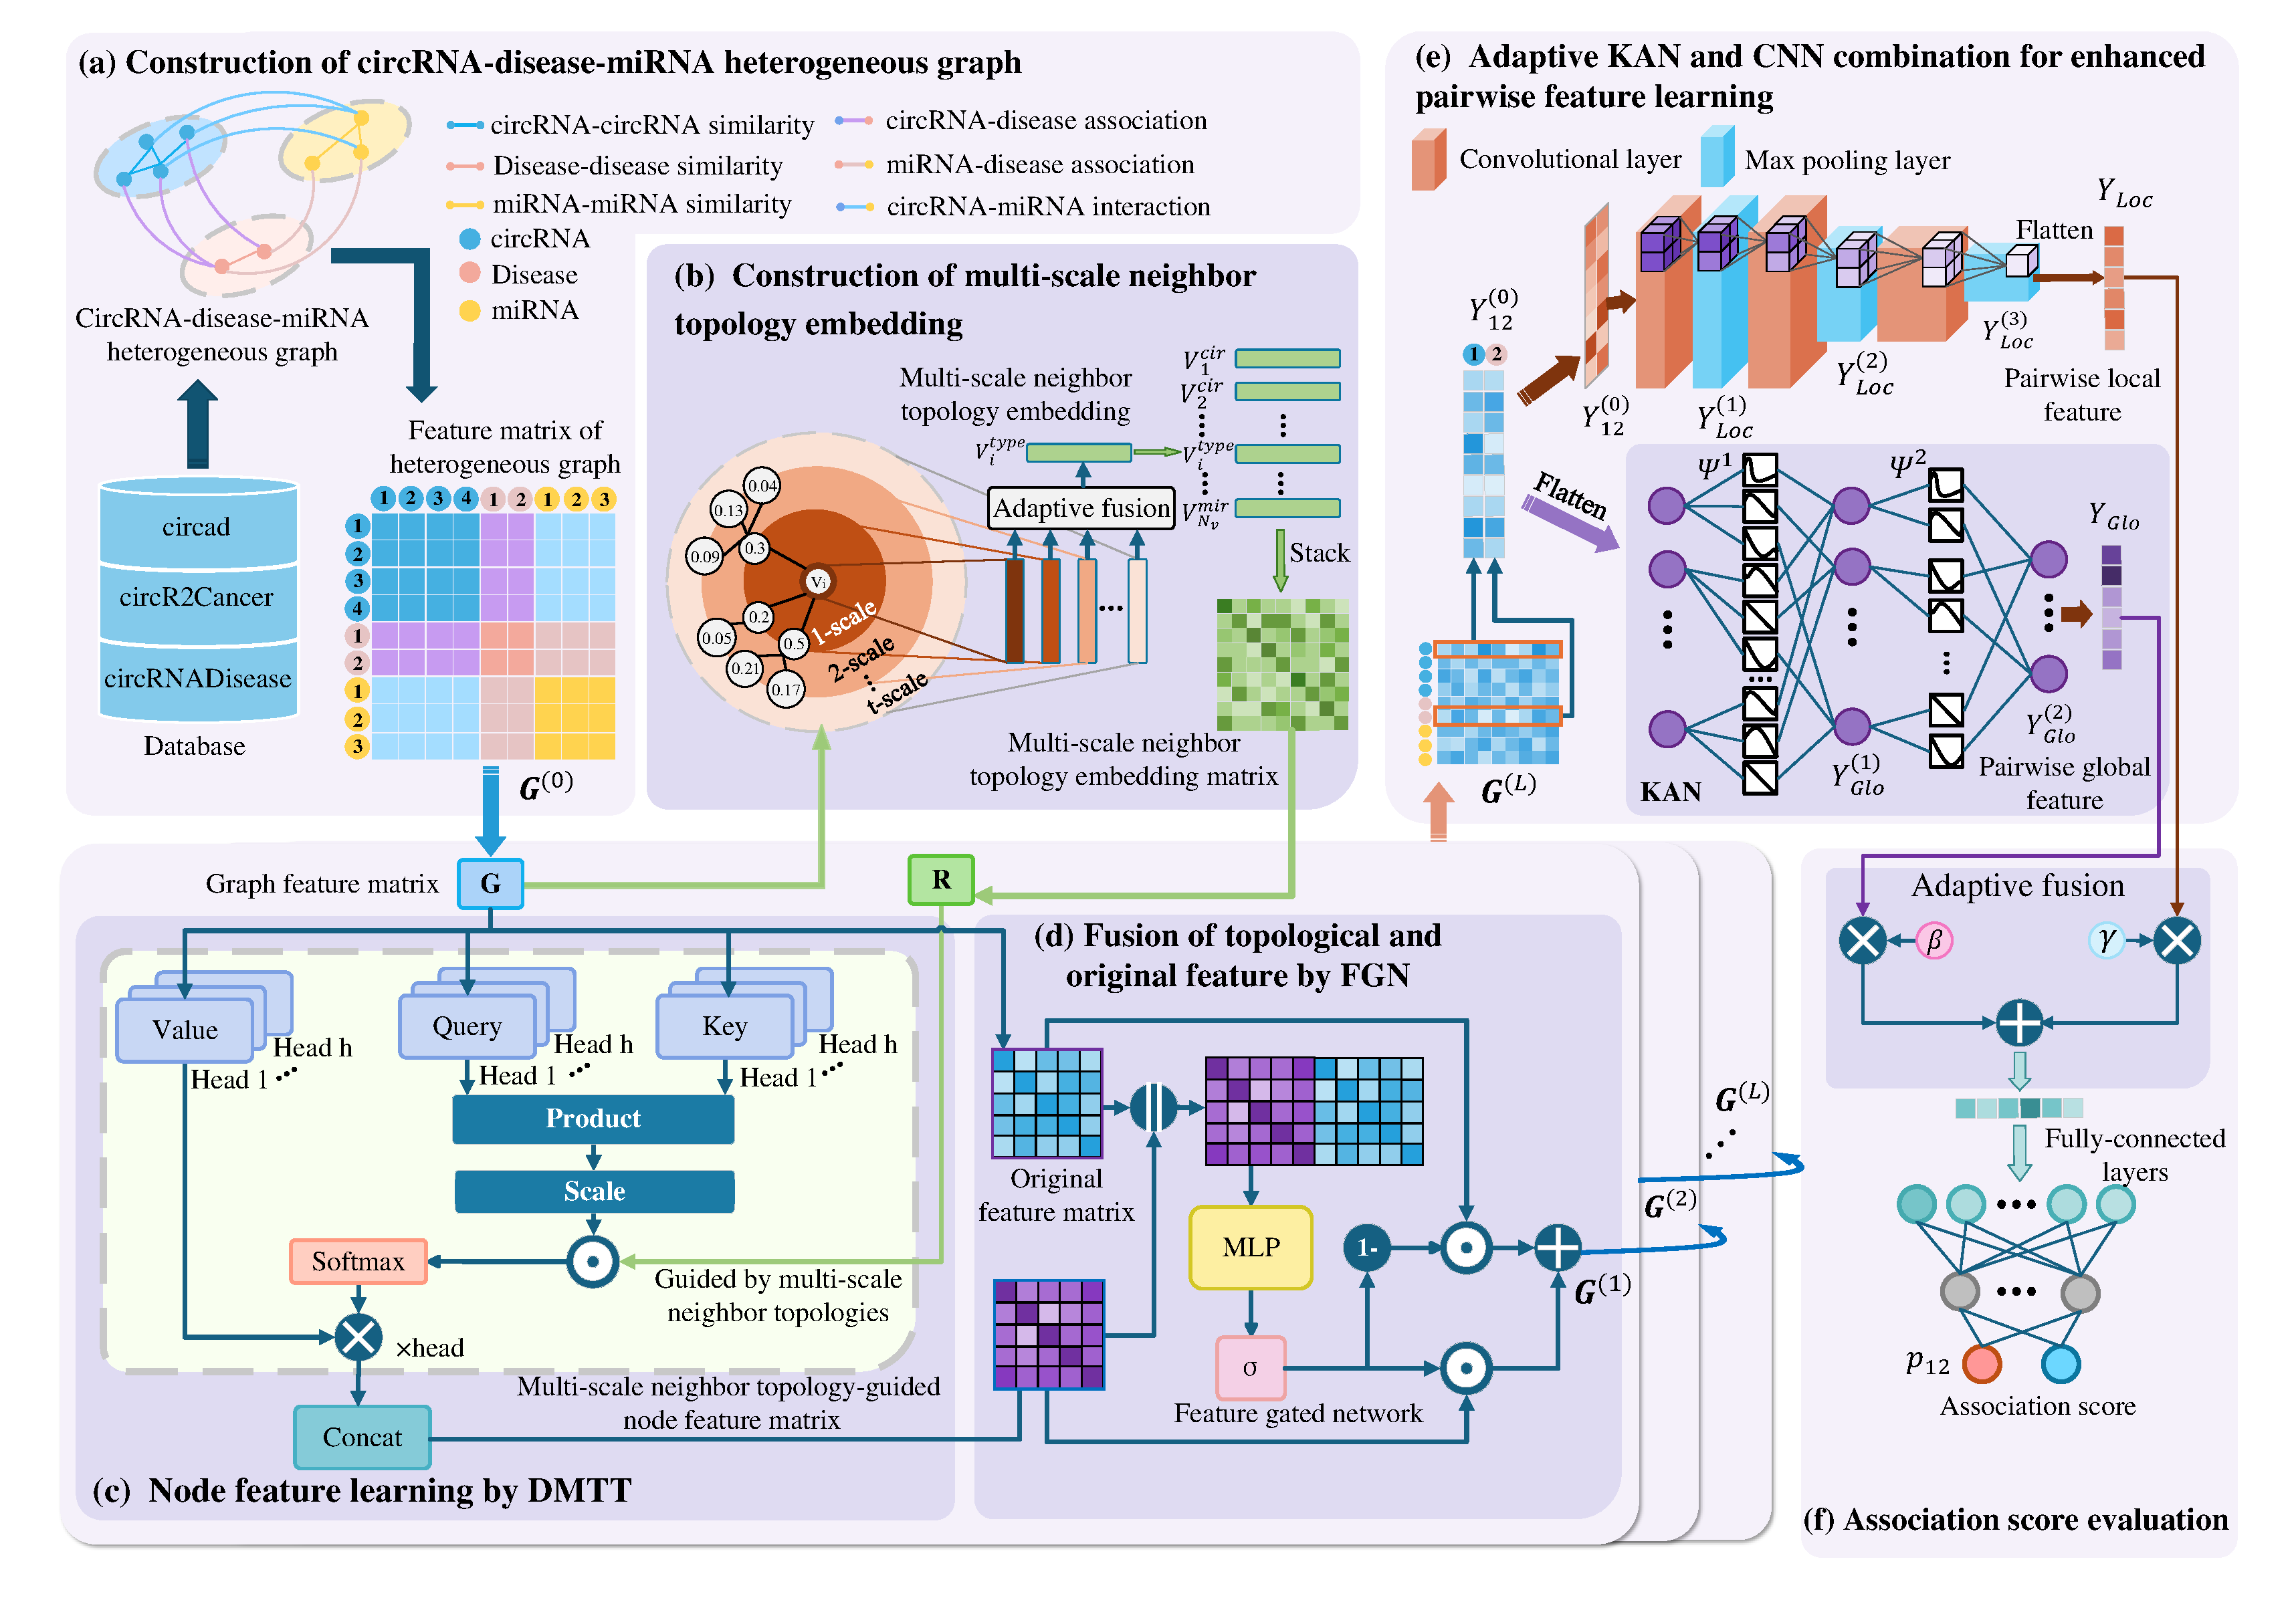
\includegraphics[width=8in]{fig/visio1.pdf}\\
	\vspace{0.2cm}
	\caption{MKCD的总体框架。(a)CircRNA-disease-miRNA 异构图的构建(b)通过ARWR构建多尺度邻居拓扑嵌入(c)基于DMTT学习circRNA、miRNA与疾病结点间的复杂关系(d)拓扑特征和结点原始特征的融合 by FGN(e)基于ACK的结点对特征局部和全局依赖性的学习(f)自适应融合两个表示来估计circRNA-disease关联分数}
	\label{fig:visio1}
	\vspace{0.1cm}
\end{figure*}


\section{Introduction}
CircRNA是一类没有5'和3'聚腺苷酸尾的单链环状非编码RNA\cite{jeck2014detecting}。越来越多的研究表明,circRNA的异常表达伴随着疾病的发生\cite{abdelmohsen2017identification},包括癌症\cite{gao2019circular,li2019tumor,liang2020autophagy}、免疫系统疾病\cite{wang2018circibtk}以及心血管疾病\cite{khan2016rbm20,siede2017identification,jin2019silencing}。因此识别特定疾病与circRNA的关联有助于疾病的诊断和治疗。计算预测方法能发现circRNAs与疾病的关联并且为后续的生物实验筛选出可靠的疾病相关的circRNA候选者\cite{lan2023benchmarking,yang2021predicting}。

现有的计算预测方法主要分为三类。第一类是建立基于网络的模型预测circRNAs与疾病的关联。KATZHCDA和PWCDA模型根据异构网络中连接它们的路径计算每个circRNA-疾病对的关联分数\cite{fan2018prediction, lei2018pwcda}。Wei et al.提出的iCircDA-MF引入了基因信息,构建circRNA-gene-disease关系网络并基于矩阵分解(matrix factorization)来进行预测\cite{wei2020icircda}。然而,这些模型受到(suffer from)有限的关联信息的阻碍。

第二类预测模型基于机器学习技术来推断circRNAs和疾病的关联。A couple of 方法结合了k-nearest neighbors来预测与疾病相关的circRNA候选\cite{wang2022combining,lei2020integrating,yan2018dwnn}。Wang et al.提出的MLCDA模型通过归纳矩阵补全(inductive matrix completion)来进行预测\cite{wang2022machine}。GBDTCDA和AE-RF都是基于决策树的预测方法\cite{lei2019gbdtcda,deepthi2021inferring},而CD-LNLP和RNMFLP则通过标签传播计算circRNA和疾病的关联分数\cite{zhang2019predicting,peng2022rnmflp}。然而这些方法均是建立了浅层的预测模型,难于学习circRNAs与疾病之间的深层关系。

第三类侧重于开发基于深度学习策略的模型,通过提取complex和有代表性的特征进一步提高预测性能。Several方法建立基于卷积神经网络(CNN)的模型来预测疾病相关的circRNAs\cite{tian2024mamlcda,wang2020efficient,lu2020improving},然而它们忽略了多个circRNA和疾病结点间的邻居拓扑结构。Li et al.提出的Bi-SGTAR使用具有稀疏门控的编码器来推断所有circRNA-disease关联倾向性\cite{li2024bi}。该方法也忽略了circRNA和疾病结点所形成的拓扑结构。其他方法分别基于图卷积网络\cite{shang2024sgfccda,liu2023mpclcda,wu2022mdgf}和图注意力网络\cite{wu2023mlngcf}以及两者的组合\cite{dai2022graphcda}来学习结点的深层特征。然而这些方法面向整个图来学习各个结点的特征,忽略了一对circRNA和疾病结点特征的全局依赖的学习。

我们提出了一个新的circRNA-disease关联预测模型MKCD,用于学习邻居拓扑with mutil-scale、多个circRNA、miRNA和疾病结点之间的联系以及结点对特征的全局和局部依赖。本文的主要贡献概征述如下。
\begin{itemize}
    \item CircRNA-disease-miRNA异构图包含了circRNA、disease、miRNA结点以及他们之间的关联、互作与相似性关系。异构图中每个circRNA(disease,miRNA)结点有着多阶邻居,这些邻居与该结点的关系有着不同的紧密程度。为了区分不同尺度邻居拓扑对结点特征学习的贡献,我们提出了一个基于重启随机游走的策略(ARWR)。它能够自适应确定每个尺度邻居拓扑的重要性,并形成多尺度邻居拓扑嵌入。
    \item 先前多数的transformer只关注结点特征之间的相似性,而忽略了结点间的拓扑结构。所提出的动态多尺度邻居拓扑指导的transformer(DMTT)对多个circRNA、miRNA和疾病结点间的联系进行编码。DMTT可以形成动态演化的邻居拓扑结构并且利用邻居拓扑来评估所有circRNA、miRNA和疾病结点的重要性。
    \item 多尺度邻居拓扑指导的结点特征聚焦于利用拓扑结构的信息,而circRNA、miRNA和disease结点的原始特征则蕴含了更多的细节。我们提出一个特征门控网络(FGN),使得能够区分拓扑特征和原始特征的重要性。
    \item 一对circRNA和疾病结点的特征蕴含着局部和全局依赖性。我们提出的结点对特征学习策略ACK is powerful in 学习特征间的全局依赖 by Kolmogorov-Arnold网络(KAN)\cite{liu2024kan}和学习局部特征间的联系 by 多层CNN。对比实验表明,MKCD在预测circRNA和疾病的关联方面优于先进的方法,并且案例研究证实了我们的方法能够筛选有潜力的疾病相关circRNA候选者。
\end{itemize}



\section{Materials and methods}

\textcolor{blue}{我们提出了一个新的预测模型MKCD(Figure \ref{fig:visio1})来预测与疾病相关的circRNA候选者。构建了一个circRNA-disease-miRNA异构图来整合circRNA,disease和miRNA之间的相似性、互作性以及关联性。MKCD由三个组件组成,分别学习异构图中的不同信息。我们提出的DMTT会编码多个circRNA、disease和miRNA结点之间的复杂关系,并且通过ARWR来动态构建的多尺度邻居拓扑嵌入来指导transformer的学习。为了保留结点特征更多的细节信息,我们引了了FGN。设计的ACK将用来捕捉与融合circRNA和disease结点对特征间的全局和局部依赖性。这些组件共同发挥作用,以提高MKCD预测circRNA-disease关联的能力。}


\subsection{Dataset}

本研究所使用的数据集来自于先前的工作\cite{lan2022kgancda},其包括了两个含有circRNA和disease的数据集。第一个数据集覆盖了514个circRNA、62个疾病以及564个miRNA。第二个数据集包含了330个circRNA、79个疾病与245个miRNA之间的关联和互作。我们将这两个数据集进行了整合,形成了一个比他们大的一个新的数据集。该数据集包含了989circRNA-disease关联、837miRNA-disease关联和902circRNA-miRNA相互作用,总共覆盖了834个circRNA、138个疾病和555个miRNA。circRNA与疾病之间的关联原始来源于circR2Cancer数据库\cite{lan2020circr2cancer}、circad数据库\cite{rophina2020circad}和circRNADisease数据库\cite{zhao2018circrna}。

\begin{figure*}[t]
	\centering
	% requires \usepackage{graphicx}
	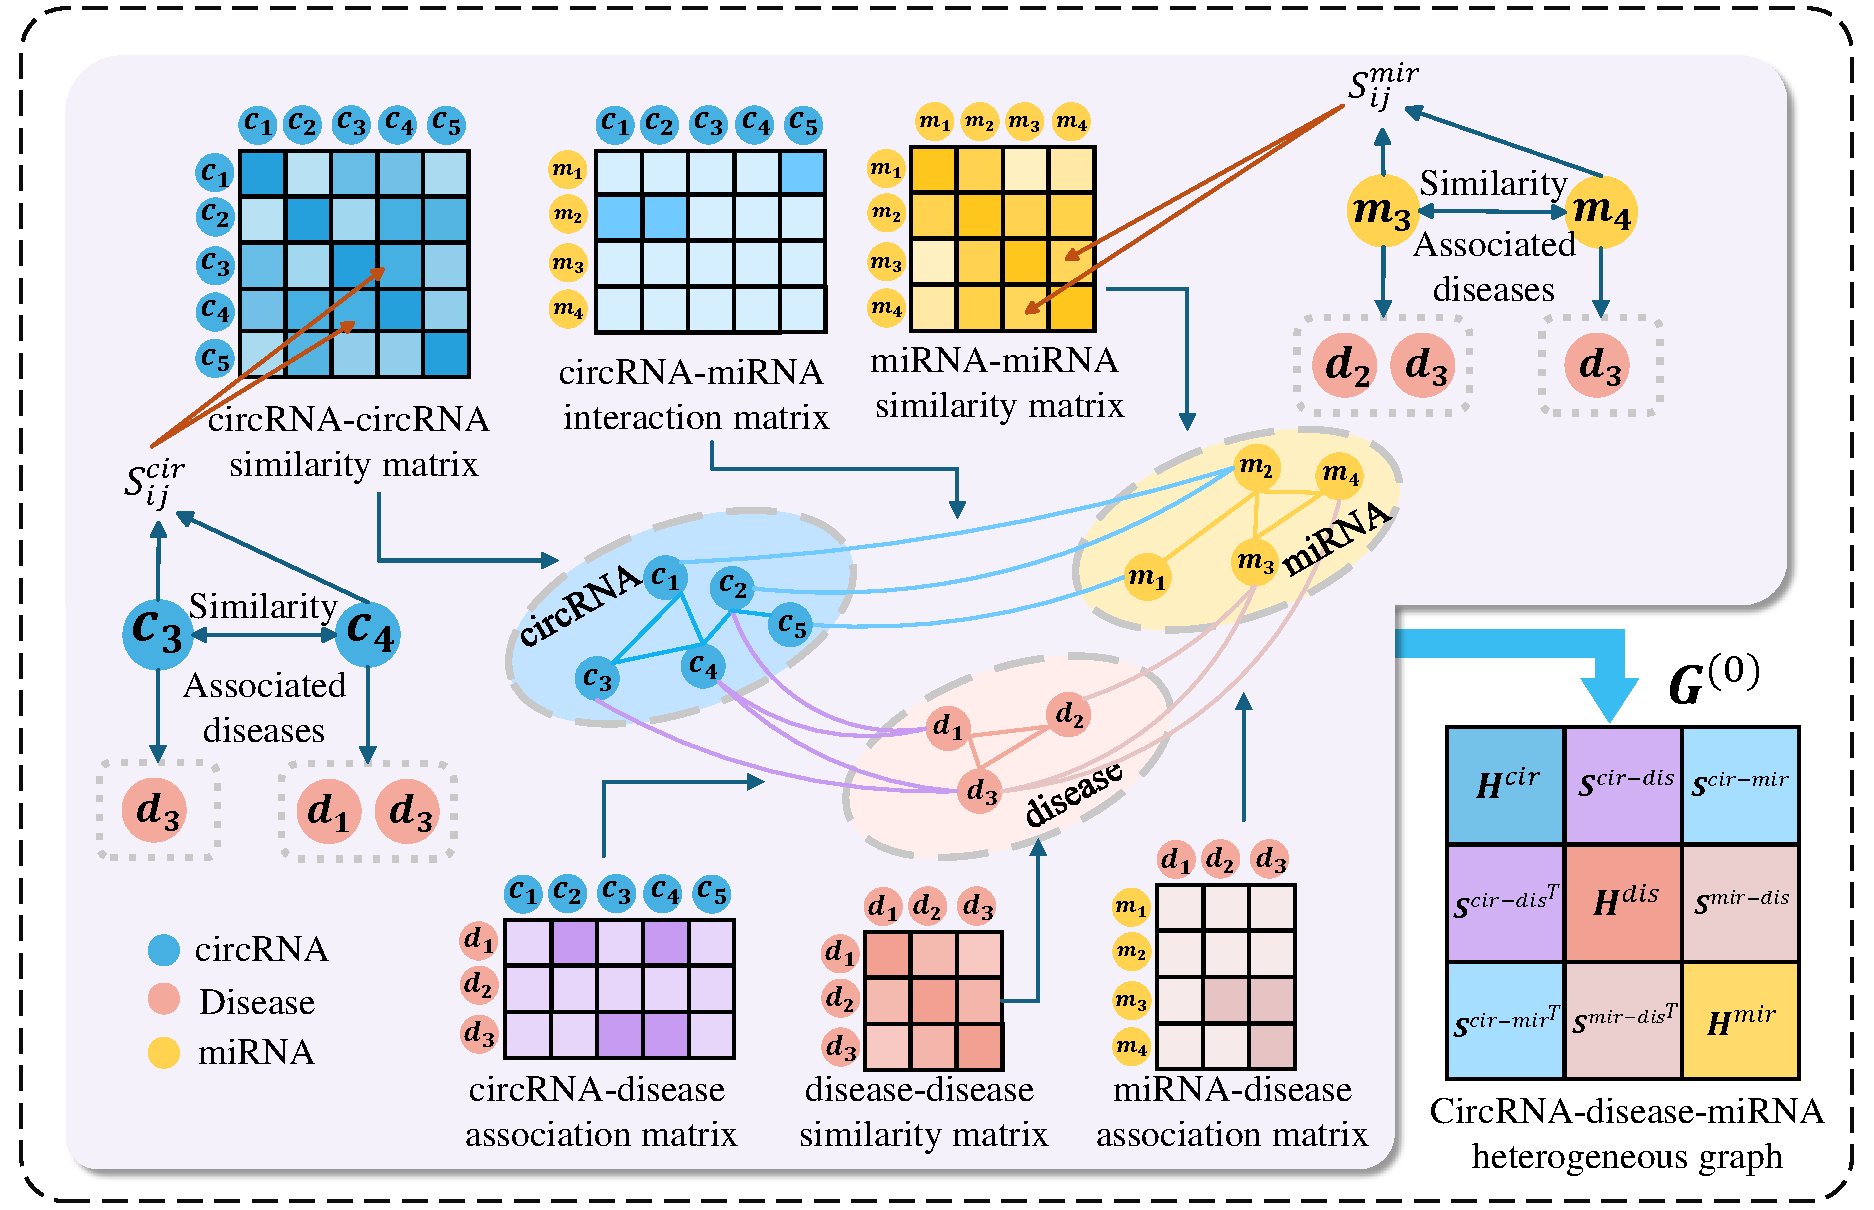
\includegraphics[width=7in]{fig/visio2.pdf}\\
	\vspace{0.2cm}
	\caption{基于多源数据的circRNA-disease-miRNA异构图构建}
	\label{fig:visio2}
	\vspace{0.1cm}
\end{figure*}

\vspace{0.3cm}


\subsection{CircRNA-disease-miRNA heterogeneous graph}
我们根据circRNA、miRNA与疾病之间的关联、互作以及相似性构建了一个三层异构图$\mathcal{G}=(\mathcal{V}, \mathcal{E})$(Figure \ref{fig:visio2})。结点集$\mathcal{V}=\{V^{cir}\cup V^{dis}\cup V^{mir}\}$包括了circRNA结点的集合$V^{cir}$,疾病结点的集合$V^{dis}$和miRNA结点的集合$V^{mir}$。边$e_{ij} \in \mathcal{E}$连接了一对结点$v_i,v_j \in \mathcal{V}$,由关联与互作矩阵$H$和相似性矩阵$S$表示。

circRNA、miRNA以及疾病间的关联与互作矩阵$H$被定义为,
\begin{equation}
H = \left\{ \begin{array}{l}
{H^{cir-dis}}\ \in {\mathbbm{R}^{N_{cir}\times N_{dis}}},if\ {v_i} \in {V^{cir}},{v_j} \in {V^{dis}};\\[5pt]
{H^{mir-dis}}\ \in {\mathbbm{R}^{N_{mir}\times N_{dis}}},if\ {v_i} \in {V^{mir}},{v_j} \in {V^{dis}};\\[5pt]
{H^{cir-mir}} \in {\mathbbm{R}^{N_{cir}\times N_{mir}}},if\ {v_i} \in {V^{cir}},{v_j} \in {V^{mir}};\\
\end{array} \right.
\end{equation}
其中$H^{cir-dis}$、$H^{mir-dis}$和$H^{cir-mir}$分别表示circRNA-disease关联矩阵、miRNA-disease关联矩阵和circRNA-miRNA相互作用矩阵。$N_{cir}$、$N_{dis}$和$N_{mir}$分别表示数据集中包含的circRNA、疾病和miRNA的数量。$H_{ij} \in H^{circ-dis} (H^{mir-dis})$表示circRNA (miRNA)结点$v_i^{cir}(v_i^{mi})$和疾病结点$v_j^{dis}$之间的关联。对于一个circRNA(mirRNA)结点 $v_i^{cir}$ ($v_i^{mir}$)和一个疾病结点$d_j^{dis}$,如果$H_{ij}^{cir-dis}=1$ ($H_{ij}^{mir-dis}=1$),则表示他们之间存在关联;反之,$H_{ij}^{cir-dis}=0$ ($H_{ij}^{mir-dis}=0$)表示没有观察到他们的关联。如果$H_{ij}^{cir-mir}=1$则表示circRNA结点$v_i^{cir}$和miRNA结点$v_j^{mir}$之间存在相互作用,否则$H_{ij}^{circ-mir}=0$。

$S$表示circRNA间的相似性、miRNA间的相似性以及疾病间的相似性矩阵,
\begin{equation}
S = \left\{ \begin{array}{l}
{S^{cir}} \in {\mathbbm{R}^{N_{cir}\times N_{cir}}},if\ {v_i},{v_j} \in {V^{cir}};\\[5pt]
{S^{dis}} \in {\ \mathbbm{R}^{N_{dis}\times N_{dis}}}\ \ ,if\ {v_i},{v_j} \in {V^{dis}}\ ;\\[5pt]
{S^{mir}} \in {\mathbbm{R}^{N_{mir}\times N_{mir}}},if\ {v_i},{v_j} \in {V^{mir}};\\[5pt]
\end{array} \right.
\end{equation}
其中$S^{cir}$、$S^{dis}$和$S^{mir}$分别是circRNA、疾病和miRNA的相似性矩阵。$S^{cir}$、$S^{dis}$和$S^{mir}$中的元素值在0到1之间,反映相同类型的两个节点之间的相似程度,元素值越高表示两个结点之间的相似度越大。

依据Wang等人\cite{wang2010inferring}的方法,一对疾病结点$[v_i^{dis},v_j^{dis}]$的相似性被计算based on他们的有向无环图(DAG)。
circRNAs和miRNAs的相似性分别通过Wang等人\cite{wang2010inferring}和Chen等人\cite{chen2015constructing}提出的方法来计算,即一对circRNAs(miRNAs)的相似性通过与它们相关联的两组疾病之间的相似性来计算得到。For instance,假设第i个circRNA结点 $v_i^{cir}$与$N_{cir}^i$个疾病关联,形成集合$\Omega_i^{cir} = \{d_{ik} | k = 1, \ldots, N_{cir}^i\}$,第j个circRNA结点 $v_j^{cir}$关联的疾病集合为$\Omega_j^{cir} = \{d_{jl} | l = 1, \ldots, N_{cir}^j\}$, $[v_i^{cir},v_j^{cir}]$的相似性$S_{ij}^{cir}$通过评估$\Omega_i^{cir}$和$\Omega_j^{cir}$之间的相似性来确定。类似的,我们可以计算得到$[v_i^{mir},v_j^{mir}]$的相似性$S_{ij}^{mir}$。

根据构建的结点间关联(互作)矩阵H和相似性矩阵S,异构图的原始特征矩阵$G^{(0)} \in \mathbb{R}^{N_v\times N_v}$被定义为,
\begin{equation}
G^{(0)} = \left[\ \begin{array}{lll}
H^{cir} & S^{cir-dis} & S^{cir-mir}\\
{S^{cir-dis}}^T & H^{dis} & {S^{mir-dis}}^T\\
{S^{cir-mir}}^T & S^{mir-dis} & H^{mir}\\
\end{array} \right],
\end{equation}
其中$N_v$为是所有circRNA、miRNA和疾病的总数,${S^{cir-dis}}^T$ 表示为矩阵$S^{cir-dis}$的转置。矩阵$G^{(0)}$的第i行$g_i$代表结点$v_i \in \mathcal{V}$的结点嵌入,其中包含了$v_i$与所有circRNA、疾病和miRNA之间的关联和相似性。$\{g_i | 0 \leqslant  i < N_{cir}\}$表示所有circRNA的结点嵌入的集合。此外,集合$\{g_i | N_{cir} \leqslant  i < N_{cir} + N_{dis}\}$和$\{g_i | N_{cir} + N_{dis} \leqslant  i < N_{cir} + N_{dis} + N_{mir}\}$分别是所有疾病和所有miRNA的结点嵌入集合。

\vspace{0.3cm}



\subsection{Construction of multi-scale neighborhood topology embedding}
circRNA-disease-miRNA异构图中的结点$v_i$具有一跳能够直接到达的一阶邻居,或者是经过$d\ (d > 1)$跳能够到达的$d$阶邻居。这些邻居结点所形成的多尺度拓扑结构,能够为circRNA与disease的关联预测提供重要的辅助信息。低阶(一阶)邻居与高阶($d$阶)邻居对于每个结点所学习到的特征有着不同的贡献,因此我们设计了ARWR来建立多尺度邻居拓扑嵌入(Figure \ref{fig:visio3})。以$v_i$为例,walker会以$v_i$作为起点出发,在circRNA-disease-miRNA异构图中进行随机游走。$v_i$在$t$时刻到达所有circRNA、disease和miRNA结点的概率分布为$\theta _i{(t)} \in \mathbb{R}^{1 \times N_v}$,
\begin{equation}
\theta _i{(t)} = (1 - \lambda) O^T \theta _i{(t-1)} + \lambda \theta _i{(0)},
\end{equation}
其中$\theta _i{(t)}$的第$j$个元素值代指walker从起点$v_i$出发经过$t$跳到达结点$v_j$$(0 \leqslant j < N_v)$的概率。$\theta _i{(0)}$是初始one-hot向量,其第$i$个位置值为1,其余均为0。$\lambda$为walker从起点重新出发的概率,$\lambda$的值越大,walker在网络当中游走的范围就越小。$O\in \mathbb{R}^{N_v\times N_v}$是$G^{(0)}$经过行归一化后得到的,其中 $o_{ij}\in O$表示walker从$v_i$转移到结点$v_j$的概率。$\theta _i{(t)}$可以被看成$v_i$经过$t$跳邻居能够到达各个结点的概率分布,因此它是$v_i$的$t$阶邻居拓扑嵌入。

经过上述过程,我们可以得到0到t阶的邻居拓扑嵌入。这些尺度的邻居拓扑嵌入被自适应地融合,得到$v_i$的多尺度邻居拓扑嵌入$\theta _i$,
\begin{equation}
\theta _i = \eta_0  \theta _i{(0)} + \eta_1 \theta _i{(1)} + \cdot \cdot \cdot + \eta_k \theta _i{(k)} + \cdot \cdot \cdot + \eta_t \theta _i{(t)},
\end{equation}
其中$\eta_k\in (0, 1)$是随机初始化的可学习参数,并且$\sum_{k=0}^{t}\eta_k = 1$。


\begin{figure}[t]
	\centering
	% requires \usepackage{graphicx}
	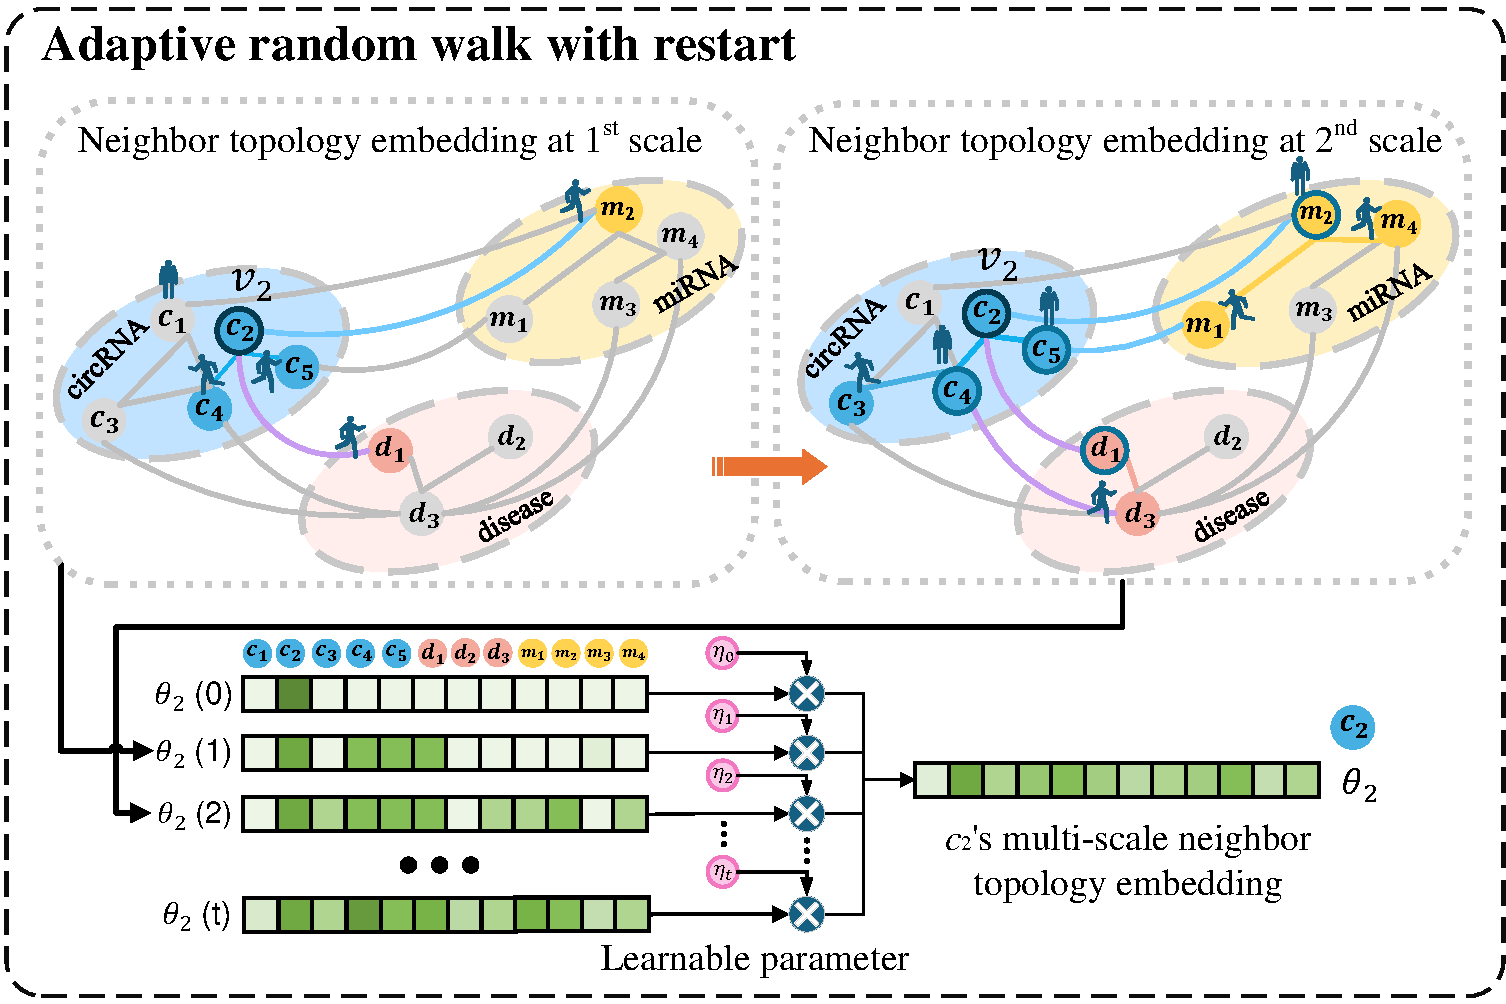
\includegraphics[width=4in]{fig/visio3.pdf}\\
	\vspace{0.2cm}
	\caption{基于ARWR构建多尺度邻居拓扑嵌入的图示(Illustration of)}
	\label{fig:visio3}
	\vspace{0.1cm}
\end{figure}



我们以每个结点作为起点进行随机游走后,可以得到的每一个结点的多尺度邻居嵌入$\theta _i$$(0\leqslant i<N_v)$。所有结点的多尺度邻居拓扑嵌入被垂直堆叠起来,形成嵌入矩阵$R \in \mathbb{R}^{N_v\times N_v}$,
\begin{equation}
	R = \left[\begin{array}{cccc}
		\theta _0\\
		\theta _1\\
		\vdots\\
		\theta _{N_v-1}
	\end{array}\right].
\end{equation}


\vspace{0.1cm}


\subsection{Node feature learning based on DMTT}
通常多个circRNA和miRNA之间会形成相互作用,并且他们会协同参与到多个疾病的过程。因此多个circRNA、miRNA和疾病结点的特征之间存在紧密联系,有必要建立自注意力机制来学习这些联系。传统transformer只聚焦于结点特征之间的相似性,没有充分exploit结点间形成的拓扑结构,尤其是多尺度的邻居拓扑结构。受到Vaswani等人\cite{vaswani2017attention}提出的transformer的启发,我们提出了动态多尺度邻居拓扑指导的transformer,利用ARWR建立的多尺度邻居拓扑嵌入来引导注意力分数的学习。

我们引入多头注意力机制,来克服单头注意力在训练过程容易陷入局部最优的问题,这有助于减少学习过程的偏差。对于第$m$个注意力头,我们首先建立查询矩阵$Q_{m}^{(l)} \in \mathbb{R}^{N_v \times \frac{N_v}{h}}$、键矩阵$K_{m}^{(l)} \in \mathbb{R}^{N_v \times \frac{N_v}{h}}$和值矩阵$V_{m}^{(l)} \in \mathbb{R}^{N_v \times \frac{N_v}{h}}$,
\begin{equation}
	\begin{aligned}
		{Q_{m}^{(l)}} &= G^{{(l - 1)}}{W_{m}^{Q{(l)}}} \\
		{K_{m}^{(l)}} &= G^{{(l - 1)}}{W_{m}^{K{(l)}}} \ \ ,\\
		{V_{m}^{(l)}} &= G^{(l - 1)}{W_{m}^{V{(l)}}}
	\end{aligned}
\end{equation}
其中$G^{(l - 1)} \in \mathbb{R}^{N_v \times N_v}$为第$l(1\leqslant l\leqslant L)$层初始输入的图结点特征矩阵。当$l = 1$时,$G^{(0)}$表示原始特征矩阵,$h$是注意力头数。$Q_{m}^{(l)}$、$K_{m}^{(l)}$和$V_{m}^{(l)}$分别是$G^{(l - 1)}$经过不同的线性投影得到的,$W_{m}^{Q{(l)}}$,$W_{m}^{K{(l)}}$,$W_{m}^{V(l)} \in \mathbb{R}^{N_v \times \frac{N_v}{h}}$为对应线性投影的权重矩阵。然后,我们对$Q_{m}^{(l)}$和${K_{m}^{(l)}}^T$进行点乘操作,得到注意力分数矩阵${S_{m}^{(l)}} \in \mathbb{R}^{N_v \times N_v}$,
\begin{equation}
	{S_{m}^{(l)}} = \frac{Q_{m}^{(l)}{K_{m}^{(l)}}^T}{\sqrt{d} },
\end{equation}
其中$d = \frac{N_v}{h}$,$\sqrt{d}$为缩放因子,用于缩放注意力分数的大小以增强训练过程中的数值稳定性。$S_{m}^{(l)}$的第$i$行记录了$v_i$与所有circRNA、疾病与miRNA结点之间的注意力分数。

在进行第$l-1$层DMTT后,结点间的拓扑结构发生了变化,依据$G^{(l - 1)}$重新通过ARWR构建得到每个结点的新的多尺度邻居拓扑嵌入$R^{(l)}$。$R^{(l)}$第$i$行记录了经过$l-1$层自注意编码后,$v_i$与其他所有circRNA、疾病与miRNA结点之间的邻居拓扑,将其与$S_{m}^{(l)}$中的第$i$行进行Hadamard乘积运算。这种做法能够使得多尺度邻居拓扑嵌入引导注意力分数的学习。我们建立多尺度邻居拓扑指导的注意力分数矩阵$\widetilde{S}_{m}^{(l)} \in \mathbb{R}^{N_v \times N_v}$,
\begin{equation}
	\widetilde{S}_{m}^{(l)} = S_{m}^{(l)}\odot R^{(l)},
\end{equation}
其中$\odot$代表Hadamard乘积运算。$\widetilde{S}_{m}^{(l)}$与$V_{m}^{(l)}$相乘将得到第$m$个注意力头所学习到的结点特征${Z_{m}^{(l)}} \in \mathbb{R}^{N_v \times \frac{N_v}{h}}$,
\begin{equation}
	{Z_{m}^{(l)}} = softmax(\widetilde{S}_{m}^{(l)})V_{m}^{(l)}.
\end{equation}
最终,通过连接$h$个注意力头各自学习到的节点特征得到第$l$层输出的多尺度邻居拓扑指导的结点特征矩阵$\hat{G}^{(l)} \in \mathbb{R}^{N_v \times N_v}$,
\begin{equation}
	\hat{G}^{(l)}= \bigg\|_{\substack{i\in {[1,h]}}} Z^{(l)}_{m},
\end{equation}
其中$\|$表示为concatenation操作。$\hat{G}^{(l)}$中的第$i$行记录了第$l$层学习到的$v_i$的特征。


\subsection{Fusion of multiple types of features based on FGN}
DMTT中,第$l$层输入的特征矩阵${G}^{(l - 1)}$蕴含了各个结点更多的细节信息,而基于DMTT学习得到的特征矩阵$\hat{G}^{(l)}$更关注经过多尺度邻居拓扑嵌入指导下的信息,因此有必要将${G}^{(l - 1)}$补充到第$l$层特征的学习中。为了融合$\hat{G}^{(l)}$和$G^{(l - 1)}$的蕴含的信息,我们在第$l$层DMTT中建立一个特征级门控,它的权重矩阵为$\alpha^{(l)}$,
\begin{equation}
	\alpha^{(l)} = \sigma (W^{gate(l)}(\hat{G}^{(l)}\| G^{(l - 1)}) + b^{gate(l)}),
\end{equation}
其中$W^{gate(l)}$和$b^{gate(l)}$为可学习的权重矩阵和偏置项,$\sigma$为Sigmoid激活函数。门控的所有参数是随机初始化的,并且在训练过程中是可学习的,因此,它可以自发地分辨出$\hat{G}^{(l)}$和$G^{(l - 1)}$中更重要的特征。

经过特征门控增强的结点特征表示为${G}^{(l)} \in \mathbb{R}^{N_v \times N_v}$,
\begin{equation}
	{G}^{(l)} =  \alpha^{(l)} \odot \hat{G}^{(l)} + (1 - \alpha^{(l)}) \odot G^{(l - 1)}.
\end{equation}
当$l \neq  L$时,$G^{(l)}$将作为下一层DMTT的输入,而$l = L$时,$G^{(L)}$是最终的结点特征表示矩阵。


\subsection{Adaptive KAN and CNN combination enhanced pairwise feature learning}
如果circRNA结点$v_i^{cir}$和疾病节点$d_j^{dis}$分别都与相同的circRNA、疾病和 miRNA 具有相似性、关联性或相互作用,则这对结点$[v_i^{cir},d_j^{dis}]$更有可能存在关联。基于这一生物学前提,我们将circRNA和疾病结点的带有门控增强的DMTT机制学习得到的特征表示上下堆叠,形成结点对级的特征表示${Y_{ij}^{(0)}} \in \mathbb{R} ^{2 \times N_v}$,
\begin{equation}
	{Y_{ij}^{(0)}} = \begin{bmatrix} {G^{(L)}_i} \\ {G^{(L)}_j} \end{bmatrix},
\end{equation}
其中集合$\{G^{(L)}_{i} | 0 \leqslant  i < N_{cir}\}$, $\{G^{(L)}_j | N_{cir} \leqslant j < N_{cir} + N_{dis}\}$分别表示为$G^{(L)}$中所有circRNA和疾病的结点特征表示。

我们设计的ACK(KAN和CNN的自适应联合策略)会进一步提取circRNA-disease结点对蕴含的信息。我们建立的KAN模块会以全局的视角来对成对结点表示进行学习,而卷积模块更聚焦于成对结点表示的局部信息的提取。
\vspace{-0.45cm}

\subsubsection{Pairwise global feature learning based on KAN}
KAN与多层感知机(MLP)相比,通过可学习的函数代替权重参数以及激活函数来自适应地学习神经元之间连接边的权重。这个可学习函数通常由多个样条函数叠加所得,这使得KAN网络能够更好地学习${Y_{ij}^{(0)}}$中各个特征间的复杂联系。${Y_{ij}^{(0)}}$经过多个KAN网络层可以学习得到结点对$[v_i^{cir},d_j^{dis}]$在全局视角下的特征表示。第$l(1\leqslant l\leqslant L)$层KAN层输入的结点对特征表示$Y_{Glo}^{(l - 1)}$在经过基于KAN网络的全局特征学习模块中的第$l$层后,得到Pairwise全局特征表示${Y}_{Glo}^{(l)}$,
\begin{equation}
	{Y}_{Glo}^{(l)} = KAN^{(l)}(Y_{Glo}^{(l - 1)}) = \varPsi^{(l)}(Y_{Glo}^{(l - 1)}),
\end{equation}
其中$KAN^{(l)}$表示第$l$个KAN层。当$l=1$时$Y_{Glo}^{(0)}$为原始的circRNA-disease结点对特征表示$Y_{ij}^{(0)}$。当$l=L$时,$Y_{Glo}^{(L)}$表示为最终的Pairwise全局特征表示${Y}_{Glo} \in \mathbb{R}^{1\times f}$,$f$为特征维度。$\varPsi^{(l)}$为第$l$层KAN层的可学习函数组成的矩阵,其一共有$n^{(l - 1)} \times n^{(l)}$个可学习的函数,因此$\varPsi^{(l)}$被定义为,
\begin{equation}
	\varPsi^{(l)} = \left(
	\begin{array}{cccc}
		\psi_{1,1} & \psi_{1,2} & \cdots & \psi_{1,n^{(l-1)}} \\
		\psi_{2,1} & \psi_{2,2} & \cdots & \psi_{2,n^{(l-1)}} \\
		\vdots & \vdots & \ddots & \vdots \\
		\psi_{n^{(l)},1} & \psi_{n^{(l)},2} & \cdots & \psi_{n^{(l)},n^{(l-1)}}
	\end{array}
	\right),
\end{equation}
其中$n^{(l - 1)}$与$n^{(l)}$分别表示第$l - 1$层和第$l$层的神经元个数。$\psi_{i,j}$对应着第$l$层第$i$个神经元与第$l - 1$层的第$j$个神经元之间连接边的的可学习函数。$\psi_{i,j}$由基函数和B样条函数组成,

\begin{equation}
	\psi_{i,j} = \omega_{b}b(x) + \omega_{s}spline(x),
\end{equation}
\begin{equation}
	spline(x) = \sum_{k = 1}^{n_{grid}}c_{k} B_{k},
\end{equation}
其中$b(x)性$为基函数${SiLU}$,$\omega_{b}$和$\omega_{s}$为可学习的权重参数。B样条函数$spline(x)$通过叠加$n_{grid}$个B样条基函数$B_{k}$得到,$c_{k}$为每一个$B_{k}$的可学习参数。

\vspace{-0.3cm}

\subsubsection{Pairwise local feature learning based on CNN}
我们建立了一个CNN来学习circRNA-disease结点对的局部特征。在CNN中,每一层block由一层卷积层和一层池化层组成。在第$l(1\leqslant l\leqslant D)$个block中,给定一对circRNA-disease结点对的特征表示${Y}_{Loc}^{(l - 1)}$,我们使用卷积操作提取它的Pairwise局部特征${Y}_{Loc}^{(l)}$,
\begin{equation}
{Y}_{Loc}^{(l)} = max(\mathop{\rm{\tau}}({W_{conv}^{(l)}} * {Y}_{Loc}^{(l - 1)} + {b_{conv}^{(l)}})),
\end{equation}
其中*表示卷积操作,$W_{conv}^{(l)}$和$b_{conv}^{(l)}$分别为卷积核和偏置项的集合,$\tau$是Leaky ReLU激活函数,max表示最大池化操作。$Y_{Loc}^{(0)}$为原始的circRNA-disease结点对特征表示$Y_{ij}^{(0)}$。当$l = D$时,对$Y_{Loc}^{(D)}$降维并展平得到最终的Pairwise局部特征表示$Y_{Loc}\in \mathbb{R}^{1\times f}$。
\vspace{-0.4cm}

\subsubsection{Adaptive fusion of pairwise local features and global features}
结点对的局部特征表示${Y_{Glo}}$和全局特征表示${Y_{Loc}}$对于每个circRNA(disease)结点的特征表示学习有着不同程度的重要性。我们为${Y_{Glo}}$和${Y_{Loc}}$各自分配一个可学习的权重参数$s_{\beta}$与$s_{\gamma}$,进行归一化后得到$\beta$和$\gamma$,
\begin{equation}
	\beta = \frac{e^{s_{\beta}}}{e^{s_{\beta}} + e^{s_{\gamma}}}\ , \quad \gamma = \frac{e^{s_{\gamma}}}{e^{s_{\beta}} + e^{s_{\gamma}}}\ .
	\end{equation}
最终的circRNA-disease结点对特征表示被定义为${Y}_{F} \in \mathbb{R}^{1\times f}$,
\begin{equation}
	{Y}_{F} = \beta \cdot {Y_{Loc}} + \gamma \cdot {Y_{Glo}}\ \ ,
\end{equation}
其中$\cdot$表示为标量乘法(Scalar Multiplication)。


\subsection{Association score evaluation and optimization}
我们使用全连接层来推导结点对$[v_i^{cir},d_j^{dis}]$的关联预测分数向量$p_{ij} \in \mathbb{R}^{1\times 2}$,
\begin{equation}
	p_{ij} = softmax(W_{Fin}Y_{F} + b_{Fin}),
\end{equation}
其中$W_{Fin}$和$b_{Fin}$为全连接层的权重矩阵和偏置项。$p_{ij} = [p_{pos}, p_{neg}]$,$p_{pos}$ 和 $p_{neg}$ 分别表示关联存在和不存在的可能性(possibility)。

在训练的过程中,我们采用AdamW算法和反向传播来优化我们的模型。我们使用交叉熵函数来估算模型的损失loss,
\begin{equation}
	loss = - \sum\limits_{(i,j) \in N} \left[ y_{ij} \log (p_{pos}) + (1 - y_{ij}) \log (p_{neg}) \right],
\end{equation}
其中 $N$ 表示所有circRNA-disease结点对的样本集合。$y_{ij}$ 表示circRNA结点 $v_i^{cir}$ 和疾病结点 $d_j^{dis}$ 之间的真实关联标签。当 $v_i^{cir}$ 和 $d_j^{dis}$ 之间存在关联时,$y_{ij} = 1$,否则 $y_{ij} = 0$。


\section{Experimental evaluations and discussions}
\subsection{Parameter settings}
在ARWR模块中,我们采用了0到2阶邻居拓扑来构建多尺度邻居拓扑嵌入,随机游走的重启概率$\lambda$被设置为0.7。对于DMTT模块,其层数L为2,在每一层DMTT中,注意力头数h被设置成4。Pairwise局部特征学习模块中,我们使用了三个block,头两个block中的卷积核大小为$2\times 2$,第三个block的卷积核为$1\times 2$,首个block池化层使用的窗口大小为$2\times 2$,剩下两个block的池化窗口均为$1\times 7$。Pairwise全局特征学习模块中,我们使用了2层KAN网络,神经元个数分别为1024和256,B样条函数的格点数$n_{grid}$被设置成了5。我们使用 Nvidia GeForce RTX 4060 训练 MKCD,利用 PyTorch 框架并使用 AdamW 算法对其进行优化。训练过程包括 40 个 epoch,批量大小为 32,学习率为 0.001,权重衰减为 0.0001。

\subsection{Evaluation metrics}
我们使用五折交叉验证来评估MKCD和其余比较方法的预测性能。所有已知的circRNA-disease关联被作为positive样本并随机划分为五等份,而所有未被观察到的的circRNA-disease关联被视作negative样本。在每个fold中,我们使用四份positive样本和等量的随机选择的negative样本作为训练集,剩余的一份positive样本以及没被训练的所有negative样本构成测试集。

我们选用the area under the receiver operating characteristic curve (AUC)\cite{hajian2013receiver}和 the area under the precision-recall curve (AUPR)\cite{saito2015precision}作为评估指标。每个折叠将单独计算AUC和AUPR,对这五个折叠的结果做平均计算得到最终的AUC和AUPR分数。此外,考虑到生物学家通常选择排名列表顶部的候选者来进一步验证,因此,我们计算了top k个疾病相关circRNAs的recall rate。


\subsection{Ablation experiments}
为了验证MARWR (mutil-scale neighbor topology embedding based on adaptive random walk with restart)、DMTT (dynamic multi-scale neighbor topology-guided self-attention)、FGN (feature gate network)和ACK (adaptive combined strategy of KAN and CNN)的有效性,我们进行了一系列的消融实验(Table \ref{tab:tab1})。我们分别去除MKCD中的MARWR、DMTT、FGN和ACK模块,计算相应的AUC和AUPR。我们观察到当所有模块都被保留时,完整模型MKCD取得了最好的预测性能,AUC和AUPR分别为0.947和0.271。当去除了MARWR时,AUC和AUPR分别下降3.4\%和6.8\%,这表明了多尺度邻居拓扑嵌入的引入对于提高circRNA和疾病关联预测的准确性有着关键作用。在去除DMTT以及FGN会导致AUC下降3.8\%,AUPR下降7.6\%,这证实了利用circRNA、disease和miRNA结点间形成的多尺度邻居拓扑结构来学习结点特征表示是非常必要的。完整模型比单独忽略FGN时AUC和AUPR分别提高了2.4\%和5.0\%,这表明了补充细节特征有利于结点特征的学习。最后,当去除ACK时,AUC和AUPR分别下降了1.6\%和3.1\%,这些结果证明了Pairwise局部特征和全局特征的自适应融合对于circRNA-disease关联预测性能提升的有效性。

消融实验的结果指明DMTT对于circRNA-disease关联预测做出了最大贡献,这主要因为DMTT编码了多个circRNA、disease和miRNA结点特征间的联系。MARWR对于模型贡献第二大(contributed the second most to the results),这是因为MARWR能够有效地引入多尺度邻居拓扑嵌入到结点特征学习。


\begin{table}[!t]
	\label{tab:01}
    \centering
    \begin{threeparttable}[b]
        \vspace{0.4cm}
        \caption{Results of ablation experiments of MKCD.}\label{tab:tab1}
        \begin{tabular}{m{1.8cm}<{\centering}m{1.2cm}<{\centering}m{1.1cm}<{\centering}m{1.1cm}<{\centering}|m{1.2cm}<{\centering}m{1.5cm}<{\centering}}
            \hline
            \textbf{MARWR} &\textbf{DMTT} & \textbf{FGN} & \textbf{ACK} & \textbf{Average AUC} & \textbf{Average AUPR} \\
            \hline
            \ding{55} &\checkmark & \checkmark & \checkmark & 0.913 & 0.203 \\
            \checkmark &\ding{55} & \ding{55} & \checkmark & 0.909 & 0.195 \\
            \checkmark &\checkmark & \ding{55} & \checkmark & 0.923 & 0.221 \\
            \checkmark &\checkmark & \checkmark & \ding{55} & 0.931 & 0.240 \\
            \checkmark &\checkmark & \checkmark & \checkmark & \textbf{0.947} & \textbf{0.271} \\
            \hline
        \end{tabular}
    \end{threeparttable}
    \vspace{-0.4cm}
\end{table}

\subsection{Comparison with other methods}
\begin{figure*}[!t]
    \centering
    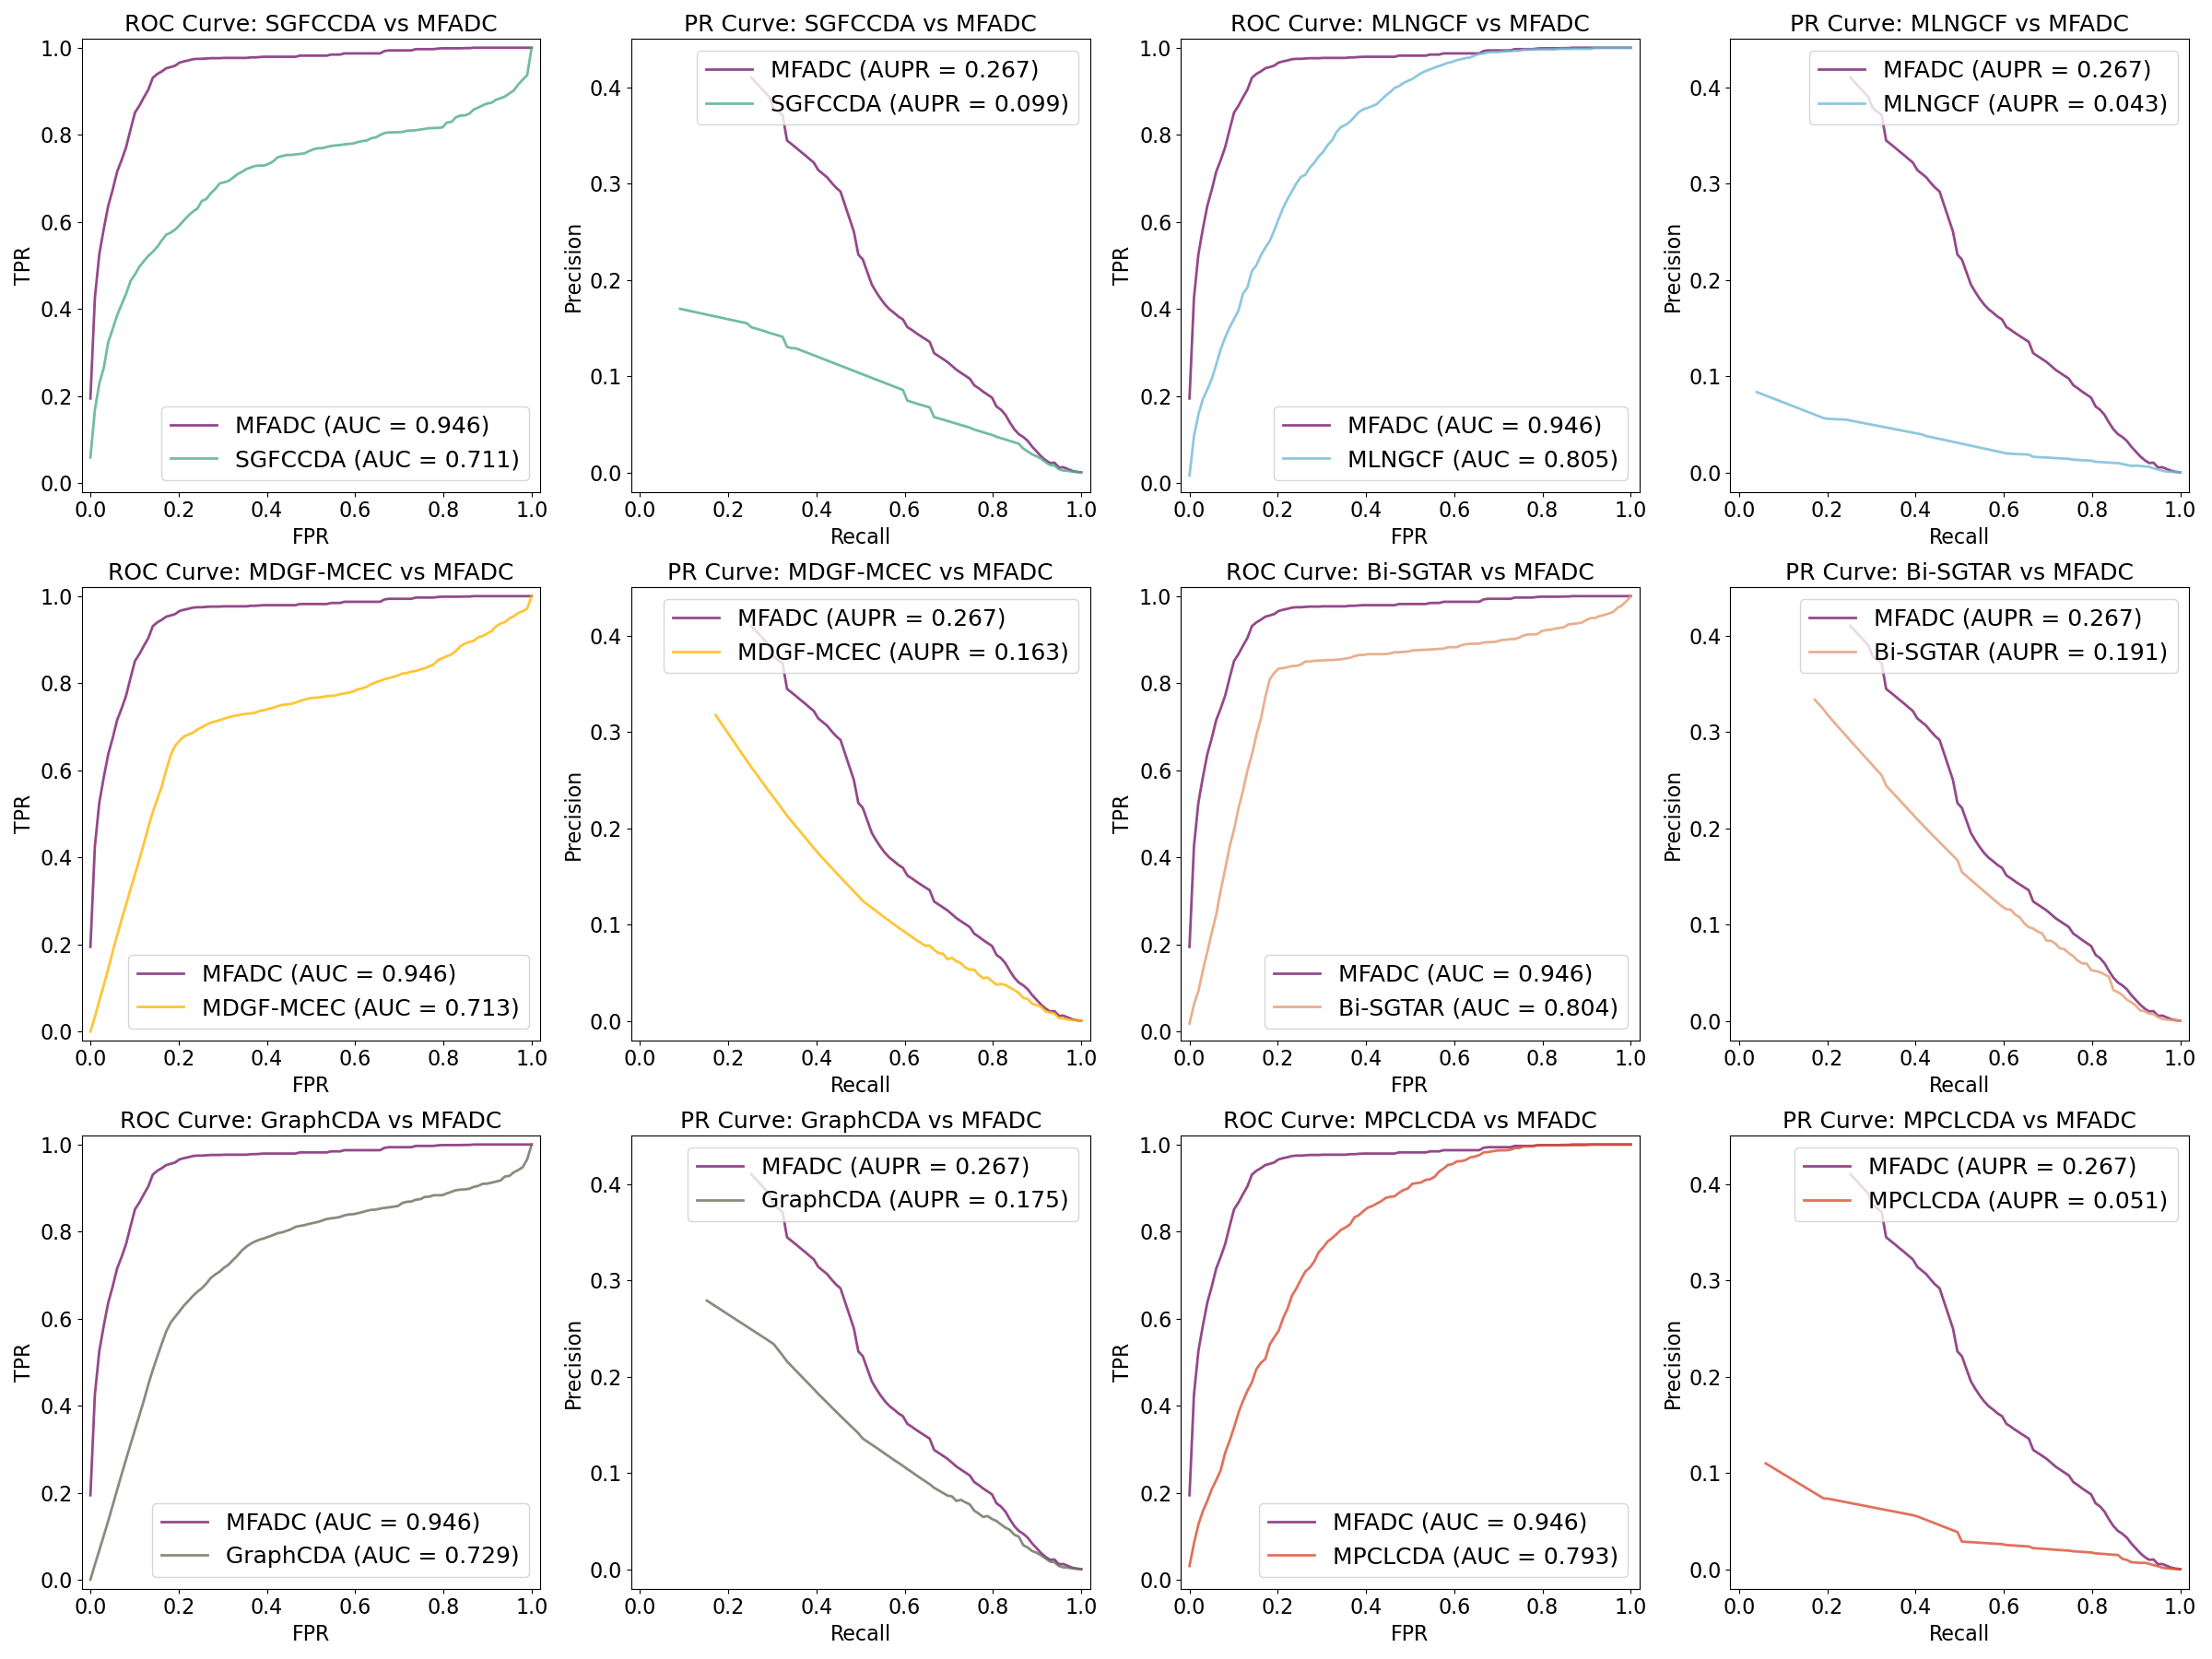
\includegraphics[width=8in]{fig/roc_pr_split.png}
    \caption{ROC and PR curves of MKCD and other methods.}
    \label{fig:roc_pr_split}
\end{figure*}

\begin{table*}[!t]
	\label{tab:02}
	\centering
	\begin{threeparttable}[b]
		\vspace{0.4cm}
		\renewcommand{\arraystretch}{1.3}  % 增大行高
		\caption{Results of the paired Wilcoxon test by comparing MKCD and any of the other methods.  }\label{tab:tab2}
        \setlength{\tabcolsep}{0pt}  % 调整列间距,适当增加空白
		\begin{tabular}{p{3.0cm}<{\centering}  p{2.9cm}<{\centering} p{2.9cm}<{\centering} p{2.9cm}<{\centering} p{2.9cm}<{\centering} p{2.9cm}<{\centering} p{2.9cm}<{\centering}}
			\hline
            \textbf{$p\ $-value} & \textbf{SGFCCDA} & \textbf{MLNGCF} & \textbf{MDGF-MCEC} &  \textbf{Bi-SGTAR} & \textbf{GraphCDA} & \textbf{MPCLCDA}\\
			\hline
		    AUC & 2.71e-111 & 7.20e-58 & 2.13e-109 &  3.27e-60 & 6.06e-108 & 1.22e-76 \\
		    AUPR & 6.02e-109 & 6.60e-115 & 1.18e-41 &  1.96e-09 & 2.86e-26 & 1.29e-113 \\
			\hline
		\end{tabular}
	\end{threeparttable}
	\vspace{-0.1cm}
\end{table*}


我们比较了MKCD和六个用来预测circRNA与疾病关联的advanced方法,包括SGFCCD\cite{shang2024sgfccda}、MLNGCF\cite{wu2023mlngcf}、\ MDGF\ -\ MCEC\cite{wu2022mdgf}、\ Bi-SGTAR\cite{li2024bi}、\ GraphCDA\cite{dai2022graphcda}\ \ 和\\MPCLCDA\cite{liu2023mpclcda}。每个方法都采用原始论文中提供的最优参数来进行训练,并且在交叉验证中使用了与MKCD相同的训练集和测试集来保证公平。

SGFCCDA: 这个模型建立了circRNA-disease异构图,并且通过尺度图卷积网络(scale graph convolutional networks)和卷积网络( convolution network)来预测潜在的circRNA-disease关联。

MLNGCF:在这个模型中,利用circRNA和疾病的多种相似性,基于多层注意力神经网络(multilayer attention neural)来估算circRNA和disease的关联分数。

MDGF-MCEC:该方法根据circRNA和疾病各自的相似性分别建立了circRNA和疾病的关系图,通过多视图双注意力图卷积网络(multi-view dual attention graph convolution network)来学习结点特征。

Bi-SGTAR:circRNA-disease异构图的邻接矩阵被分解成两个视图,并采用具有稀疏门控的编码器来识别所有circRNA-disease关联。

GraphCDA:This approach 分别建立了circRNA相似网络和疾病相似网络,It utilizes图卷积网络和图注意力网络相结合的混合图嵌入模型来同时学习circRNA和疾病的特征表示。

MPCLCDA:它自动挑选元路径用于构建元路径图,并利用图卷积网络和对比学习来学习circRNA和疾病结点特征。

Figure \ref{fig:roc_pr_split}展示了MKCD和其他方法的ROC和PR曲线。从图中可以看出,MKCD在获得了最高的平均AUC,为0.947,超过SGFCCDA 23.5\%,MLNGCF 14.1\%,MDGF-MCEC 23.3\%,Bi-SGTAR 14.2\%,GraphCDA 21.7\%和MPCLCDA 15.3\%。MKCD的平均AUPR为0.271,分别比SGFCCDA、MLNGCF、MDGF-MCEC、Bi-SGTAR、GraphCDA和MPCLCDA高 17.2\%、22.8\%、10.8\%、8.0\%、9.6\%、22.0\%。MLNGCF和MPCLCDA都使用了图神经网络,仅聚焦在融合circRNA-disease异构图的拓扑和结点特征,因此它们取得了较差的结果。与这两个方法相比,SGFCCDA则使用尺度图卷积网络来克服图卷积网络的线性层结构导致不同通道之间特征混合的问题,于是它取得了更好的性能。MDGF-MCEC和GraphCDA主要着眼于多个相似性视图的学习,而Bi-SGTAR则聚焦于多个异构图视图的学习,这使得他们都具有更高的AUPR。我们的方法优于这六个方法主要因为嵌入了多尺度邻居拓扑和编码了多个circRNA、disease和miRNA结点特征之间的联系。


对于所有138个疾病上的预测结果,我们使用了配对Wilcoxon检验来评估我们方法的性能是否显著高于其他六个方法。根据Table \ref{tab:tab2}的结果,所有的$p$-value均小于0.05,这表明MKCD在AUC和AUPR方面的性能显著优于SGFCCDA、MLNGCF、MDGF-MCEC、Bi-SGTAR、GraphCDA和MPCLCDA。


对于每个疾病,我们计算了circRNA候选者在不同top $k$ value下召回率(Figure \ref{fig:topK})。当$k = 30$,MKCD获得了29.3\%的召回率,surpassing SGFCCDA 12.1\%,MLNGCF 15.2\%,MDGF-MCEC 8.1\%,Bi-SGTAR 8.0\%,GraphCDA 9.1\%,MPCLCDA 15.1\%。当$k$=50, 70, 90时,MKCD保持着领先的位置,召回率分别为48.5\%、68.6\%和90.1\%。Bi-SGTAR(41.3\%、65.7\%、89.8\%)、MDGF-MCEC(41.3\%、63.6\%、87.9\%)和GraphCDA(39.4
\%、62.5\%、88.8\%)也取得了decent的性能。SGFCCDA(29.3\%、45.5\%、70.6\%)、MLNGCF(25.2\%、39.4\%、64.6\%)和MPCLCDA(25.3\%、40.5\%、66.7\%)则取得了inferior的性能。

 
% \begin{figure*}[t]
%     \centering
%     % requires \usepackage{graphicx}
%     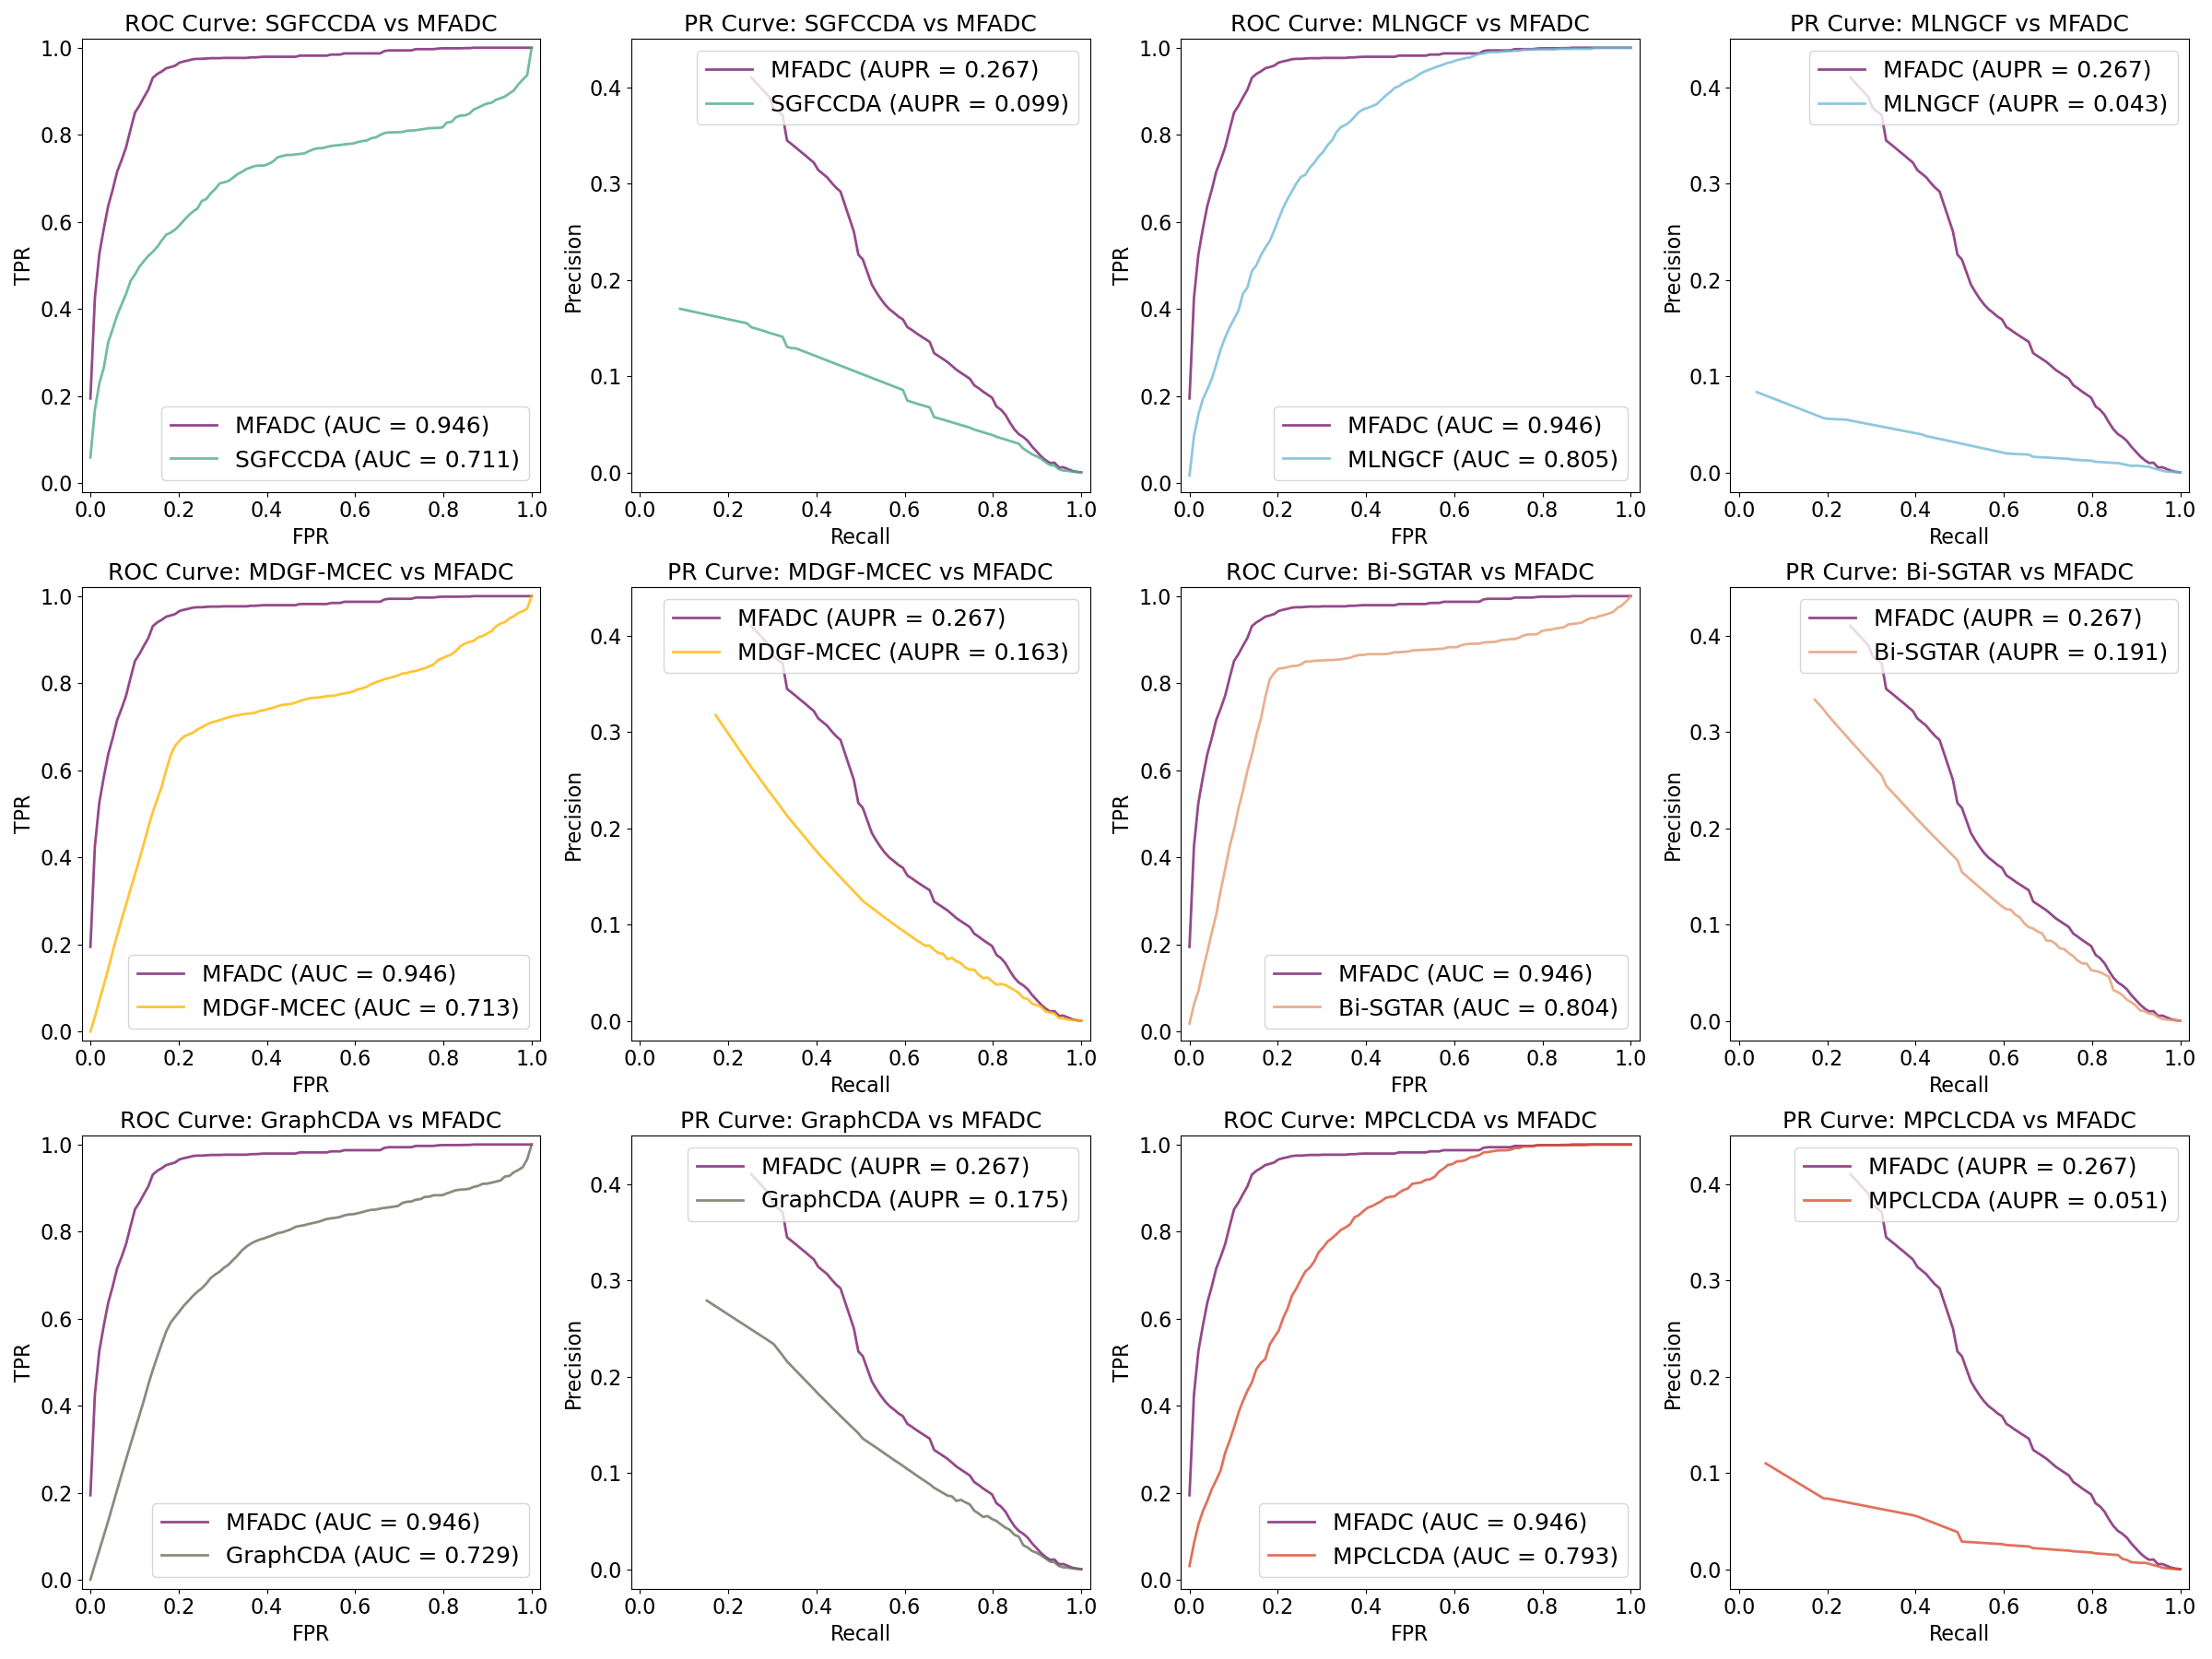
\includegraphics[width=8in]{fig/roc_pr_split.png}\\
%     \vspace{0.2cm}
%     \caption{compare...... }
%     \label{fig:compare}
%     \vspace{0.1cm}
% \end{figure*}

% \begin{figure*}[t]
%     \centering
%     % requires \usepackage{graphicx}
%     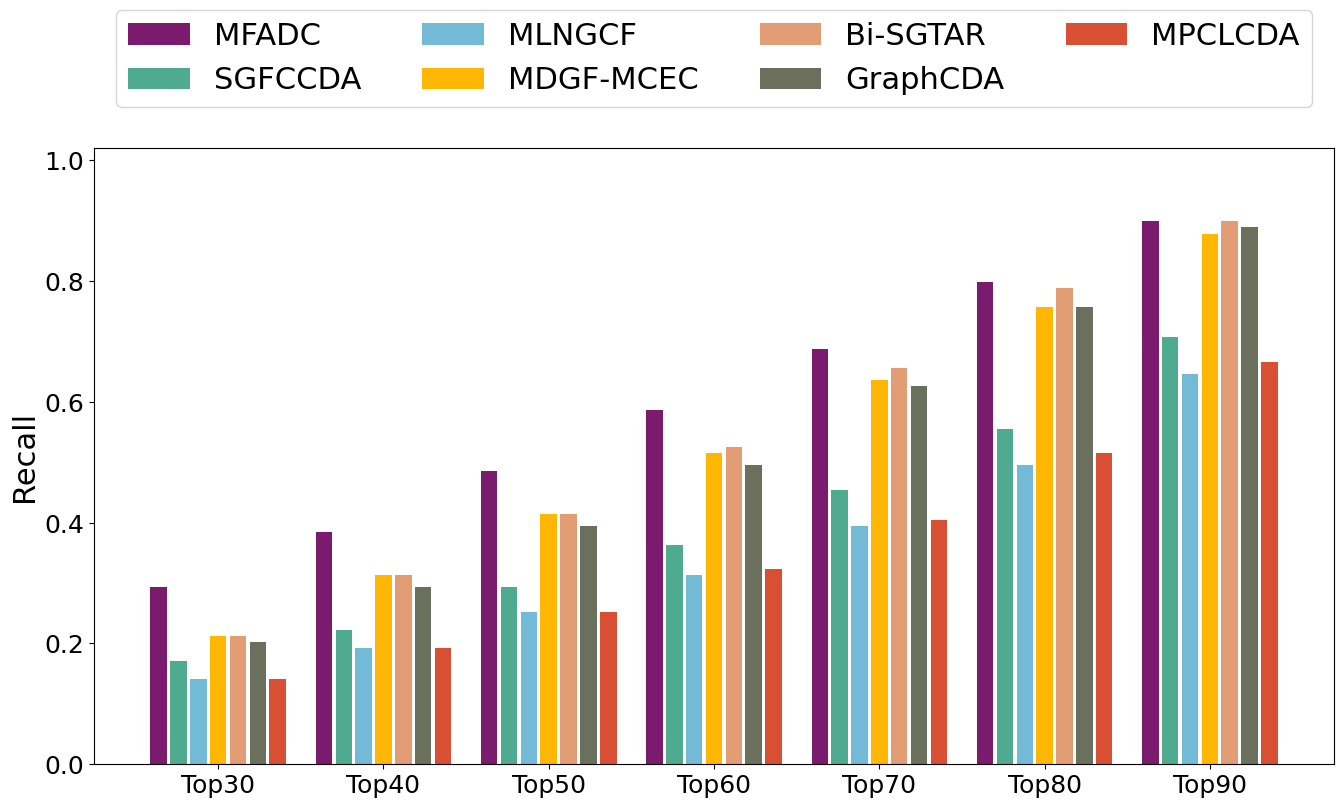
\includegraphics[width=8in]{fig/TopK_Recall.png}\\
%     \vspace{0.2cm}
%     \caption{compare...... }
%     \label{fig:topk}
%     \vspace{0.1cm}
% \end{figure*}


% \begin{table}[!t]
% 	\label{tab:02}
%     \centering
%     \begin{threeparttable}[b]
%         \vspace{0.4cm}
% 		\renewcommand{\arraystretch}{1.3}  % 增大行高
% 		\caption{Average AUCs and AUPRs of our method and the compared methods over all the 834 circRNAs.  }\label{tab:tab2}
%         \setlength{\tabcolsep}{0pt}  % 调整列间距,适当增加空白
% 		\begin{tabular}{p{4.0cm}<{\centering}  p{2.9cm}<{\centering} p{2.9cm}<{\centering}}
% 			\hline
% 			\textbf{methods} & \textbf{AUC} & \textbf{AUPR} \\
% 			\hline
% 		    SGFCCDA& 0.711 & 0.099 \\
%             MLNGCF& 0.805 & 0.043 \\
% 		    MDGF-MCEC& 0.713 & 0.163 \\
%             BiSGTAR& 0.804 & 0.191 \\
%             GraphCDA& 0.729 & 0.175 \\
%             MPCLCDA& 0.793 & 0.051 \\
%             MKCD  & \textbf{0.947} & \textbf{0.271} \\
% 			\hline
%         \end{tabular}
%     \end{threeparttable}
%     \vspace{-0.4cm}
% \end{table}





\subsection{Case studies over three diseases}

\begin{figure*}[!t]
    \centering
    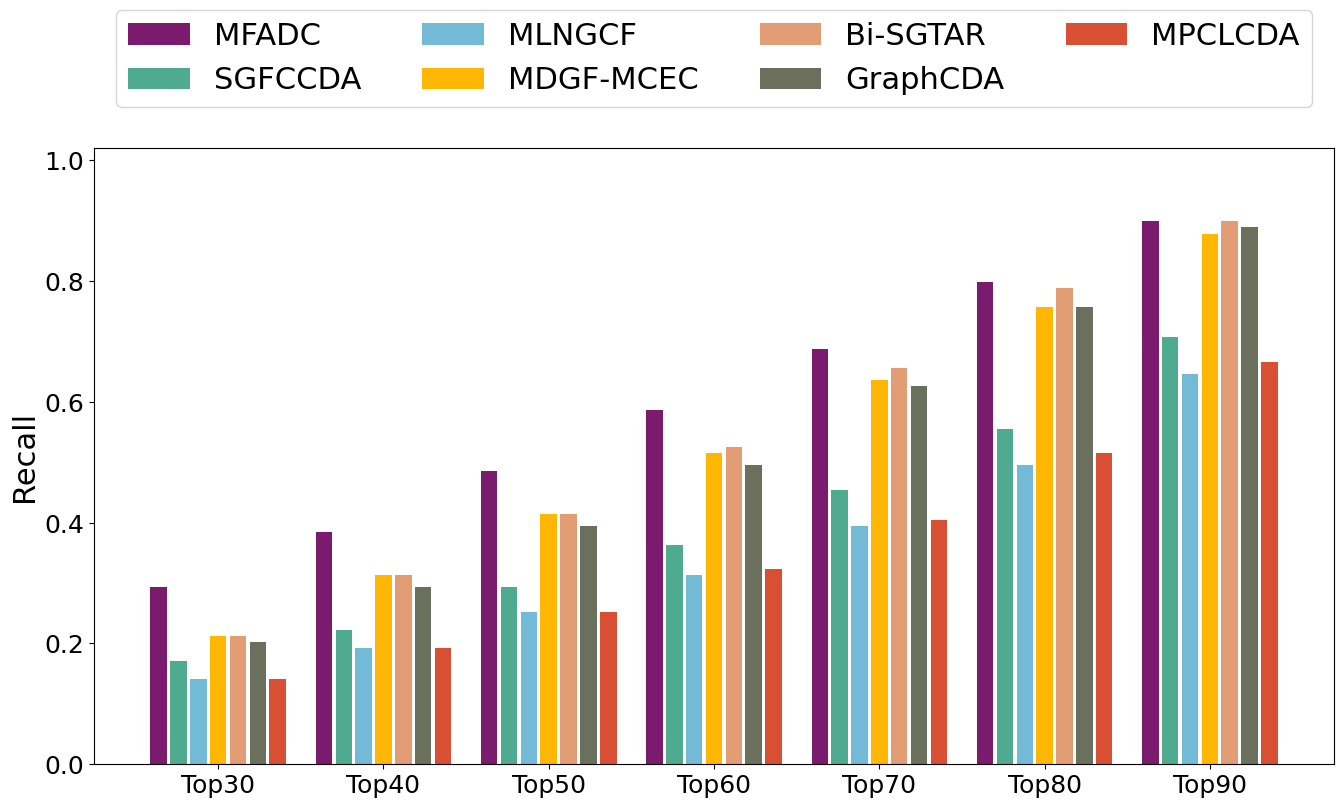
\includegraphics[width=6.5in]{fig/TopK_Recall.png}
     \caption{The average recall rates of diseases at multiple top k cutoffs}
    \label{fig:topK}
\end{figure*}

我们对glioma(神经胶质瘤)、systemic lupus erythematosus(系统性红斑狼疮)和glioblastoma(胶质母细胞瘤)进行了案例研究,进一步验证MKCD挖掘与疾病相关的潜在circRNA候选者的能力。glioma与glioblastoma是两种原发性脑肿瘤\cite{weller2015glioma,wirsching2017glioblastoma},而systemic lupus erythematosus是一种systemic autoimmune disease,affecting primarily women\cite{borchers2010geoepidemiology}。每种疾病的circRNA候选者按照关联分数降序排列,并选取前15个circRNA作为候选者。Table \ref{tab:tab3}、Table \ref{tab:tab4}和Table \ref{tab:tab5}分别展示了glioma、systemic lupus erythematosus和glioblastoma的前15个circRNA候选者。\textcolor{blue}{circRNADisease v2.0数据库提供了经过实验验证的circRNA与各种疾病之间的关联,覆盖了4246个circRNAs和330个疾病\cite{sun2024mode}。该数据库以及相关的生物信息学文献被用来验证circRNA-disease关联的预测。}

\begin{table*}[!t]
	\label{tab:03}
    \centering
    \begin{threeparttable}[b]  
        \caption{The top 15 predicted results of glioma-related circRNAs based on MKCD.}	\label{tab:tab3}
        \vspace{0.4cm}
        \setlength{\tabcolsep}{0pt}  % 调整列间距,适当增加空白
        \begin{tabular}{p{2cm}<{\centering} p{3.9cm}<{\raggedright} p{4.5cm}<{\raggedright} | p{2cm}<{\centering} p{3.9cm}<{\raggedright} p{4.2cm}<{\raggedright}}
            \hline
            \textbf{Rank} &  \textbf{circRNA name} & \textbf{Evidence} & \textbf{Rank} &  \textbf{circRNA name} & \textbf{Evidence} \\
            \hline
            1 & circ\_002136 & $L^a$, PMID:30736838 & 9 & hsa\_circ\_0079593 & $L^a$, PMID:31148222 \\
            2 & hsa\_circ\_0061868 & PMID:30341906 & 10 & circSMO742 & $L^a$, PMID:31895689 \\
            3 & circPTN & $L^a$, PMID:31511040 & 11 & hsa\_circ\_0012129 & $L^a$, PMID:29686222 \\
            4 & circ-TTBK2 & $L^a$, PMID:32196629 & 12 & hsa\_circ\_0088732 & $L^a$, PMID:32154171 \\
            5 & circ-EZH2 & $L^a$, PMID:31669648 & 13 & circNFIX & $L^a$, PMID:30072869 \\
            6 & hsa\_circ\_0000594 &  $L^a$, PMID:28219405 & 14 & circ-PTPRZ1 & $L^a$, PMID:31364003 \\
            7 & hsa\_circ\_0005198 & $L^a$, PMID:31038801 & 15 & hsa\_circ\_0014359 & $L^a$, PMID:30745107 \\
            8 & hsa\_circ\_0000177 & $L^a$, PMID:30010402 & & & \\
            \hline
        \end{tabular}
        \begin{tablenotes}
            \item $L^a$: circRNADisease v2.0.
        \end{tablenotes}
    \end{threeparttable}
    \vspace{-0.4cm}
\end{table*}

\begin{table*}[!t]
	\label{tab:04}
    \centering
    \begin{threeparttable}[b]  
        \caption{The top 15 predicted results of systemic lupus erythematosus-related circRNAs based on MKCD.}	\label{tab:tab4}
        \vspace{0.4cm}
        \setlength{\tabcolsep}{0pt}  % 调整列间距,适当增加空白
        \begin{tabular}{p{2cm}<{\centering} p{3.9cm}<{\raggedright} p{4.5cm}<{\raggedright} | p{2cm}<{\centering} p{3.9cm}<{\raggedright} p{4.2cm}<{\raggedright}}
            \hline
            \textbf{Rank} &  \textbf{circRNA name} & \textbf{Evidence} & \textbf{Rank} &  \textbf{circRNA name} & \textbf{Evidence} \\
            \hline
            1 & hsa\_circ\_0046599 & $L^a$, PMID:29360436 & 9 & hsa\_circ\_0008615 & $L^a$, PMID:29360436 \\
            2 & hsa\_circ\_0001866 & $L^a$, PMID:29360436 & 10 & hsa\_circ\_0021549 & $L^a$, PMID:29360436 \\
            3 & hsa\_circ\_0034398 & $L^a$, PMID:29360436 & 11 & has\_circ\_0049220 & $L^a$, PMID:29606700 \\
            4 & hsa\_circ\_0003146 & $L^a$, PMID:29360436 & 12 & hsa\_circ\_0092374 & $L^a$, PMID:29360436 \\
            5 & hsa\_circ\_0000479 & $L^a$, PMID:31608065 & 13 & hsa\_circ\_0040705 & $L^a$, PMID:29360436 \\
            6 & hsa\_circ\_0057762 & $L^a$, PMID:30628013 & 14 & hsa\_circ\_0012919 & $L^a$, PMID:30237316 \\
            7 & circPTPN22 & $L^a$, PMID:30871426 & 15 & hsa\_circ\_0049224 & $L^a$, PMID:29606700 \\
            8 & hsa\_circ\_0045272 & $L^a$, PMID:29700819 & & & \\
            \hline
        \end{tabular}
        \begin{tablenotes}
            \item $L^a$: circRNADisease v2.0.
        \end{tablenotes}
    \end{threeparttable}
    \vspace{-0.4cm}
\end{table*}

\begin{table*}[!t]
	\label{tab:05}
    \centering
    \begin{threeparttable}[b]  
        \caption{The top 15 predicted results of glioblastoma-related circRNAs based on MKCD.}	\label{tab:tab5}
        \vspace{0.4cm}
        \setlength{\tabcolsep}{0pt}  % 调整列间距,适当增加空白
        \begin{tabular}{p{2cm}<{\centering} p{3.9cm}<{\raggedright} p{4.5cm}<{\raggedright} | p{2cm}<{\centering} p{3.9cm}<{\raggedright} p{4.2cm}<{\raggedright}}
            \hline
            \textbf{Rank} &  \textbf{circRNA name} & \textbf{Evidence} & \textbf{Rank} &  \textbf{circRNA name} & \textbf{Evidence} \\
            \hline
            1 & hsa\_circ\_0001801 & $L^a$, PMID:31858556 & 9 & circMTO1 & $L^a$, PMID:31456594 \\
            2 & circNT5E & $L^a$, PMID:29967262 & 10 & circ-AKT3 & $L^a$, PMID:31470874 \\
            3 & circ-PITX1 & $L^a$, PMID:31493405 & 11 & circPVT1 & unknown \\
            4 & hsa\_circ\_0043949 & $L^a$, PMID:31823158 & 12 & circPTN & $L^a$, PMID:31511040 \\
            5 & hsa\_circ\_0074027 & $L^a$, PMID:30738578 & 13 & hsa\_circ\_101996 & unknown \\
            6 & circMMP9 & $L^a$, PMID:30470262 & 14 & hsa\_circ\_100242 & unknown \\
            7 & circ-Foxo3 & $L^a$, PMID:31802888 & 15 & hsa\_circ\_0003855 & unknown \\
            8 & hsa\_circ\_0001946 & $L^a$, PMID:31599076 & & & \\
            \hline
        \end{tabular}
        \begin{tablenotes}
            \item $L^a$: circRNADisease v2.0.
        \end{tablenotes}
    \end{threeparttable}
    \vspace{-0.4cm}
\end{table*}

以glioma为例(Table \ref{tab:tab3}),15个circRNAs均得到了文献的证实,\textcolor{blue}{并且其中的14个在circRNADisease v2.0中被发现}。例如,排名第一位的hsa\_circ\_002136由He等人\cite{he2019fus}发现其会抑制U87胶质瘤暴露的内皮细胞(GECs)的存活、迁移和管形成。排名第二位的hsa\_circ\_0061868则经过Li等人\cite{li2019circ}的研究发现其在胶质瘤中的表达水平上调(the expression levels of chsa\_circ\_0061868 ... were upregulated)。

前15个与systemic lupus erythematosus\ (SLE)相关的circRNA候选者(Table \ref{tab:tab4})均得到了文献的证实,\textcolor{blue}{且都收录在circRNADisease v2.0中}。例如,Li等人\cite{li2018comprehensive}发现hsa\_circ\_0046599可以作为系统性红斑狼疮的潜在生物标志物。hsa\_circ\_0000479由Guo等人\cite{guo2019hsa_circ_0000479}证实其在SLE患者外周血单个核细胞中上调(upregulated in peripheral blood mononuclear cells of patients with SLE)。

\textcolor{blue}{对于glioblastoma,前15个circRNA候选者(Table \ref{tab:tab5})中的11个在最近的文献以及circRNADisease v2.0中得到证实}。例如Wang等人\cite{wang2018circnt5e}的研究表明,circNT5E在胶质母细胞瘤中表现出肿瘤抑制样特征(exhibiting tumor suppressor-like features in glioblastoma)。circMMP9经由Wang等人\cite{wang2018eif4a3}证明了其会促进glioblastoma multiforme cell的增殖、迁移和侵袭能力。


\subsection{Prediction of novel circRNA-disease associations}
我们使用所有已知的circRNAs与疾病之间的关联,并随机选取等量的反例来训练MKCD,用于预测138个疾病的circRNA候选者。\href{path/to/S1.pdf}{Supplementary File S1}中列出了由MKCD预测的每个疾病的前15位circRNA候选者。


\section{Conclusion}
本文介绍了一个新方法来编码出多个circRNA、miRNA和疾病结点特征间的联系,并对结点对的全局和局部特征进行学习与整合,以预测疾病相关的circRNAs。通过调整随机游走者在circRNA-disease-miRNA异构图中的行走范围来形成多个尺度的邻居拓扑,并且各阶邻居拓扑的重要性被自适应地确定。设计的多尺度邻居拓扑指导的transformer能够动态更新邻居拓扑,并学习多个circRNA、miRNA和疾病结点特征间的动态联系。特征层面的门控网络被建立来为更重要拓扑特征和原始特征分配更高的权重。提出的ACK编码了circRNA-dsease结点对的特征,其有助于揭示pairwise属性之间的局部和全局依赖性。五折交叉验证实验结果展示了MKCD的AUC和AUPR高于对比的六个方法。top-ranked circRNA候选者的召回率和三个疾病的案例研究表明MKCD有能力提供可靠的疾病相关的circRNA候选。




\end{methods}

% \setlength{\fboxrule}{1pt}
\begin{thebibliography}{}
\normalsize
%1
\bibitem{jeck2014detecting}
Jeck W R, Sharpless N E. Detecting and characterizing circular RNAs. Nature biotechnology, 2014, 32(5): 453-461.
%2
\bibitem{holdt2018molecular}
Holdt L M, Kohlmaier A, Teupser D. Molecular roles and function of circular RNAs in eukaryotic cells. Cellular and Molecular Life Sciences, 2018, 75(6): 1071-1098.
%3
\bibitem{liu2022circular}
Liu C X, Chen L L. Circular RNAs: Characterization, cellular roles, and applications. Cell, 2022, 185(12): 2016-2034.
%4
\bibitem{abdelmohsen2017identification}
Abdelmohsen K, Panda A C, Munk R, et al. Identification of HuR target circular RNAs uncovers suppression of PABPN1 translation by CircPABPN1. RNA biology, 2017, 14(3): 361-369.
%5
\bibitem{gao2019circular}
Gao S, Yu Y, Liu L, et al. Circular RNA hsa\_circ\_0007059 restrains proliferation and epithelial-mesenchymal transition in lung cancer cells via inhibiting microRNA-378. Life sciences, 2019, 233: 116692.
%6
\bibitem{li2019tumor}
Li Z, Ruan Y, Zhang H, et al. Tumor‐suppressive circular RNAs: mechanisms underlying their suppression of tumor occurrence and use as therapeutic targets. Cancer science, 2019, 110(12): 3630-3638.
%7
\bibitem{liang2020autophagy}
Liang G, Ling Y, Mehrpour M, et al. Autophagy-associated circRNA circCDYL augments autophagy and promotes breast cancer progression. Molecular cancer, 2020, 19: 1-16.
%8
\bibitem{wang2018circibtk}
Wang X, Zhang C, Wu Z, et al. CircIBTK inhibits DNA demethylation and activation of AKT signaling pathway via miR-29b in peripheral blood mononuclear cells in systemic lupus erythematosus. Arthritis Research \& Therapy, 2018, 20: 1-10.
%9
\bibitem{khan2016rbm20}
Khan M A F, Reckman Y J, Aufiero S, et al. RBM20 regulates circular RNA production from the titin gene. Circulation research, 2016, 119(9): 996-1003.
%10
\bibitem{siede2017identification}
Siede D, Rapti K, Gorska A A, et al. Identification of circular RNAs with host gene-independent expression in human model systems for cardiac differentiation and disease. Journal of molecular and cellular cardiology, 2017, 109: 48-56.
%11
\bibitem{jin2019silencing}
Jin C, Zhao W, Zhang Z, et al. Silencing circular RNA circZNF609 restrains growth, migration and invasion by up-regulating microRNA-186-5p in prostate cancer. Artificial cells, nanomedicine, and biotechnology, 2019, 47(1): 3350-3358.
%12
\bibitem{lan2023benchmarking}
Lan W, Dong Y, Zhang H, et al. Benchmarking of computational methods for predicting circRNA-disease associations. Briefings in Bioinformatics, 2023, 24(1): bbac613.
%
\bibitem{yang2021predicting}
Yang J, Lei X. Predicting circRNA-disease associations based on autoencoder and graph embedding. Information Sciences, 2021, 571: 323-336.
%13
\bibitem{fan2018prediction}
Fan C, Lei X, Wu F X. Prediction of CircRNA-disease associations using KATZ model based on heterogeneous networks. International journal of biological sciences, 2018, 14(14): 1950.
%14
\bibitem{lei2018pwcda}
Lei X, Fang Z, Chen L, et al. PWCDA: path weighted method for predicting circRNA-disease associations. International journal of molecular sciences, 2018, 19(11): 3410.
%14
\bibitem{wei2020icircda}
Wei H, Liu B. iCircDA-MF: identification of circRNA-disease associations based on matrix factorization. Briefings in bioinformatics, 2020, 21(4): 1356-1367.
%15
\bibitem{wang2022combining}
Wang M N, Xie X J, You Z H, et al. Combining K nearest neighbor with nonnegative matrix factorization for predicting circrna-disease associations. IEEE/ACM Transactions on Computational Biology and Bioinformatics, 2022, 20(5): 2610-2618.
%
\bibitem{lei2020integrating}
Lei X, Bian C. Integrating random walk with restart and k-Nearest Neighbor to identify novel circRNA-disease association. Scientific reports, 2020, 10(1): 1943.
%16
\bibitem{yan2018dwnn}
Yan C, Wang J, Wu F X. DWNN-RLS: regularized least squares method for predicting circRNA-disease associations. BMC bioinformatics, 2018, 19: 73-81.
%16
\bibitem{wang2022machine}
Wang L, Wong L, Li Z, et al. A machine learning framework based on multi-source feature fusion for circRNA-disease association prediction. Briefings in Bioinformatics, 2022, 23(5): bbac388.
%17
\bibitem{lei2019gbdtcda}
Lei X, Fang Z. GBDTCDA: predicting circRNA-disease associations based on gradient boosting decision tree with multiple biological data fusion. International journal of biological sciences, 2019, 15(13): 2911.
%
\bibitem{deepthi2021inferring}
Deepthi K, Jereesh A S. Inferring potential CircRNA–disease associations via deep autoencoder-based classification. Molecular Diagnosis \& Therapy, 2021, 25: 87-97.
%18
\bibitem{peng2022rnmflp}
Peng L, Yang C, Huang L, et al. RNMFLP: predicting circRNA–disease associations based on robust nonnegative matrix factorization and label propagation. Briefings in bioinformatics, 2022, 23(5): bbac155.
%
\bibitem{zhang2019predicting}
Zhang W, Yu C, Wang X, et al. Predicting CircRNA-disease associations through linear neighborhood label propagation method. Ieee Access, 2019, 7: 83474-83483.
%
\bibitem{tian2024mamlcda}
Tian Y, Zou Q, Wang C Y, et al. MAMLCDA: A Meta-Learning Model for Predicting circRNA-Disease Association Based on MAML Combined With CNN. IEEE Journal of Biomedical and Health Informatics, 2024.
%
\bibitem{wang2020efficient}
Wang L, You Z H, Huang Y A, et al. An efficient approach based on multi-sources information to predict circRNA–disease associations using deep convolutional neural network. Bioinformatics, 2020, 36(13): 4038-4046.
%
\bibitem{lu2020improving}
Lu C, Zeng M, Wu F X, et al. Improving circRNA–disease association prediction by sequence and ontology representations with convolutional and recurrent neural networks. Bioinformatics, 2020, 36(24): 5656-5664.
%
\bibitem{li2024bi}
Li S, Chen Q, Liu Z, et al. Bi-SGTAR: A simple yet efficient model for circRNA-disease association prediction based on known association pair only. Knowledge-Based Systems, 2024, 291: 111622.
%21
\bibitem{shang2024sgfccda}
Shang J, Zhao L, He X, et al. SGFCCDA: Scale Graph Convolutional Networks and Feature Convolution for circRNA-Disease Association Prediction. IEEE Journal of Biomedical and Health Informatics, 2024.
%24
\bibitem{liu2023mpclcda}
Liu W, Tang T, Lu X, et al. MPCLCDA: predicting circRNA–disease associations by using automatically selected meta-path and contrastive learning. Briefings in Bioinformatics, 2023, 24(4): bbad227.
%23
\bibitem{wu2022mdgf}
Wu Q, Deng Z, Pan X, et al. MDGF-MCEC: a multi-view dual attention embedding model with cooperative ensemble learning for CircRNA-disease association prediction. Briefings in Bioinformatics, 2022, 23(5): bbac289.
%19
\bibitem{wu2023mlngcf}
Wu Q, Deng Z, Zhang W, et al. MLNGCF: circRNA–disease associations prediction with multilayer attention neural graph-based collaborative filtering. Bioinformatics, 2023, 39(8): btad499.
%22
\bibitem{dai2022graphcda}
Dai Q, Liu Z, Wang Z, et al. GraphCDA: a hybrid graph representation learning framework based on GCN and GAT for predicting disease-associated circRNAs. Briefings in Bioinformatics, 2022, 23(5): bbac379.
%32
\bibitem{liu2024kan}
Liu Z, Wang Y, Vaidya S, et al. Kan: Kolmogorov-arnold networks. arXiv preprint arXiv:2404.19756, 2024.
%
\bibitem{lan2022kgancda}
Lan W, Dong Y, Chen Q, {\it et al.} KGANcDA: a knowledge graph attention network for lncRNA-disease association prediction. {\it Briefings in Bioinformatics} 2022;23(1):bbab494.
%26
\bibitem{lan2020circr2cancer}
Lan W, Zhu M, Chen Q, {\it et al.} CircR2Cancer: a manually curated database of associations between circRNAs and cancers. {\it Database} 2020;2020:baaa085.
%27
\bibitem{rophina2020circad}
Rophina M, Sharma D, Poojary M, {\it et al.} CircAD: a comprehensive database for differentially expressed circRNAs associated with various diseases. {\it Database} 2020;2020:baaa019.
%28
\bibitem{zhao2018circrna}
Zhao Z, Wang K, Wu F, {\it et al.} circRNA disease: a manually curated database of experimentally supported circRNA-disease associations. {\it Cell Death \& Disease} 2018;9(5):475.
%29
\bibitem{wang2010inferring}
Wang D, Wang J, Lu M, {\it et al.} Inferring the human microRNA functional similarity and functional network based on microRNA-associated diseases. {\it Bioinformatics} 2010;26(13):1644-1650.
%30
\bibitem{chen2015constructing}
Chen X, Clarence Yan C, Luo C, {\it et al.} Constructing lncRNA functional similarity network based on lncRNA-disease associations and disease semantic similarity. {\it Scientific reports} 2015;5:11338
%31
\bibitem{vaswani2017attention}
Vaswani A. Attention is all you need. Advances in Neural Information Processing Systems, 2017.

%33
\bibitem{hajian2013receiver}
Hajian-Tilaki K. Receiver operating characteristic (ROC) curve analysis for medical diagnostic test evaluation. Caspian journal of internal medicine, 2013, 4(2): 627.
%34
\bibitem{saito2015precision}
Saito T, Rehmsmeier M. The precision-recall plot is more informative than the ROC plot when evaluating binary classifiers on imbalanced datasets. PloS one, 2015, 10(3): e0118432.
%
\bibitem{weller2015glioma}
Weller M, Wick W, Aldape K, et al. Glioma. Nature reviews Disease primers, 2015, 1(1): 1-18.
%
\bibitem{wirsching2017glioblastoma}
Wirsching H G, Weller M. Glioblastoma. Malignant Brain Tumors: State-of-the-Art Treatment, 2017: 265-288.
%
\bibitem{borchers2010geoepidemiology}
Borchers A T, Naguwa S M, Shoenfeld Y, et al. The geoepidemiology of systemic lupus erythematosus. Autoimmunity reviews, 2010, 9(5): A277-A287.
%35
\bibitem{sun2024mode}
Sun Z Y, Yang C L, Huang L J, et al. circRNADisease v2.0: an updated resource for high-quality experimentally supported circRNA-disease associations. Nucleic Acids Research, 2024, 52(D1): D1193-D1200.
%
\bibitem{he2019fus}
He Z, Ruan X, Liu X, et al. FUS/circ\_002136/miR-138-5p/SOX13 feedback loop regulates angiogenesis in Glioma. Journal of Experimental \& Clinical Cancer Research, 2019, 38: 1-19.
%36
\bibitem{li2019circ}
Li G, Huang M, Cai Y, et al. Circ‐U2AF1 promotes human glioma via derepressing neuro‐oncological ventral antigen 2 by sponging hsa‐miR‐7‐5p. Journal of Cellular Physiology, 2019, 234(6): 9144-9155.
%37
\bibitem{li2018comprehensive}
Li H, Li K, Lai W, et al. Comprehensive circular RNA profiles in plasma reveals that circular RNAs can be used as novel biomarkers for systemic lupus erythematosus. Clinica Chimica Acta, 2018, 480: 17-25.
%38
\bibitem{guo2019hsa_circ_0000479}
Guo G, Wang H, Ye L, et al. Hsa\_circ\_0000479 as a novel diagnostic biomarker of systemic lupus erythematosus. Front Immunol 10: 2281.(2019)
%39
\bibitem{wang2018circnt5e}
Wang R, Zhang S, Chen X, et al. CircNT5E acts as a sponge of miR-422a to promote glioblastoma tumorigenesis. Cancer research, 2018, 78(17): 4812-4825.
%40
\bibitem{wang2018eif4a3}
Wang R, Zhang S, Chen X, et al. EIF4A3-induced circular RNA MMP9 (circMMP9) acts as a sponge of miR-124 and promotes glioblastoma multiforme cell tumorigenesis. Molecular cancer, 2018, 17: 1-12.
\end{thebibliography}

\end{document}
